\documentclass[journal]{IEEEtran}
\usepackage{amssymb}%数学符号
\usepackage{amsthm}%数学定理
\usepackage{amsmath}%数学公式、矩阵、积分求和等
\usepackage{lineno}%显示行号
\usepackage{txfonts} %默认字体times new roman
\usepackage{enumitem}%项目编号
\usepackage{multirow} %多行合并
\usepackage{caption} %改变图表标题
\usepackage{txfonts} %默认字体times new roman
\usepackage{array} %\调用公式宏包的命令应放在调用定理宏包命令之前,也能控制表格
\usepackage{booktabs} %调整表格线与上下内容的间隔
\usepackage{longtable}%调用跨页表格
\usepackage{bm}%数学字体加粗
\usepackage{setspace} %调整一段文字的行间距
\usepackage[comma, numbers,square]{natbib} %参考文献管理包
\usepackage{subfigure}
%% The amssymb package provides various useful mathematical symbols
\usepackage{amssymb}
% %% The amsthm package provides extended theorem environments
\usepackage{amsthm}
% \usepackage{ntheorem}
\counterwithout{figure}{section}%
\usepackage{threeparttable}
% \usepackage[section]{placeins}
\usepackage{afterpage}
\newtheorem{theorem}{Theorem}
\newtheorem{lemma}[theorem]{Lemma}
% \newtheorem*{proof}{Proof}
\newtheorem{remark}[theorem]{Remark}
\newtheorem{defi}[theorem]{Definition}
\newtheorem{property}[theorem]{Property}
\newtheorem{corollary}[theorem]{Corollary}
% updated with editorial comments 8/9/2021

\ifCLASSINFOpdf
   \usepackage[pdftex]{graphicx}
  % declare the path(s) where your graphic files are
  % \graphicspath{{../pdf/}{../jpeg/}}
  % and their extensions so you won't have to specify these with
  % every instance of \includegraphics
  % \DeclareGraphicsExtensions{.pdf,.jpeg,.png}
\else
  % or other class option (dvipsone, dvipdf, if not using dvips). graphicx
  % will default to the driver specified in the system graphics.cfg if no
  % driver is specified.
  %  \usepackage[dvips]{graphicx}
   \usepackage{graphicx}
  % declare the path(s) where your graphic files are
  % \graphicspath{{../eps/}}
  % and their extensions so you won't have to specify these with
  % every instance of \includegraphics
  % \DeclareGraphicsExtensions{.eps}
\fi

\hyphenation{op-tical net-works semi-conduc-tor}

\begin{document}

\title{Modeling and stability analyses of the general Connected Automated Vehicle platoon with multiple time delays}



\author{Tiancheng~Ruan,
        Hao~Wang,
        Rui~Jiang,
        Yunxue~Lu,
        Changyin~Dong,
\thanks{T. Ruan,  H. Wang, Y. Lu and C. Dong are with the
School of Transportation, Southeast University, Nanjing 211189, P.R. China;
Jiangsu Key Laboratory of Urban ITS, Southeast University, Nanjing, 210096, P.R. China;
Jiangsu Province Collaborative Innovation Center of Modern Urban Traffic Technologies, Southeast University, Nanjing, 210096, P.R. China(e-mail: ruantiancheng@seu.edu.cn;  haowang@seu.edu.cn;230198695@seu.edu.cnm;
dongcy@seu.edu.cn).}% <-this % stops a space

\thanks{R. Jiang is with Key Laboratory of Transport Industry of Big Data Application Technologies for Comprehensive Transport, Ministry of Transport, Beijing Jiaotong University, Beijing, 100044, P.R. China(e-mail: jiangrui@bjtu.edu.cn).}
% await for specific detail
\thanks{Manuscript received January 10, 2023.(Corresponding author: Hao Wang.)}}
% Remember, if you use this you must call \IEEEpubidadjcol in the second
% column for its text to clear the IEEEpubid mark.

\begin{abstract}
  Literature has shown the potential of Connected Automated Vehicles (CAVs) in improving capacity, safety, and pollutant emission.  These benefits are preconditioned to meeting stability, which is the primary goal of CAV. However, the widely used feedback control cannot guarantee stability due to the inevitable delays. Therefore, extensive research has been conducted to derive stability criteria considering delays. However, limited by the fitting model of engine dynamics, only the effect of communication delay is considered. In fact, the internal delay also significantly affects engine dynamics, where considering internal delay can significantly improve the model fit. Moreover, the methodology of stability criterion considering multiple time delays needs to be proposed. Therefore, this paper first proposes a general supermatrix representation of the CAV platoon considering multiple delays to address this issue. In addition, a novel stability criterion of the general CAV platoon considering multiple delays is derived based on Lyapunov-Krasovskii Stability Theorem and free-weighting matrix. Moreover, considering system uncertainties, another stability criterion that considers time-varying structured uncertainties is also derived. Furthermore, extensive numerical simulations are conducted in multiple scenarios to verify the effects of multiple delays, uncertainties, and control parameters on tracking performance and safety conditions. The results indicate that all CAVs under each case can track errors and return to equilibrium if the stability criteria are satisfied. Besides, the introduction of time-varying structured uncertainties and the internal communication delay worsens the tracking performance, where uncertainties lead to more significant overshoot and recovering time, while the internal communication delay makes CAV unable to perform the desired time headway. Moreover, introducing uncertainties similarly worsens the safety condition, making collision-prone scenarios more probable. Further, from the point of view of control parameters, increasing the gain of spacing and velocity errors can benefit tracking performance, while increasing the gain of acceleration errors does not.

\end{abstract}

\begin{IEEEkeywords}
  Connected and Automated Vehicles (CAVs); CAV platoon; State-space modeling; Stability analysis; Multiple time delays.
\end{IEEEkeywords}

\IEEEpeerreviewmaketitle


\section{Introduction}
\label{Section 1}
% The very first letter is a 2 line initial drop letter followed
% by the rest of the first word in caps.
% 
% form to use if the first word consists of a single letter:
% \IEEEPARstart{A}{demo} file is ....
% 
% form to use if you need the single drop letter followed by
% normal text (unknown if ever used by the IEEE):
% \IEEEPARstart{A}{}demo file is ....
% 
% Some journals put the first two words in caps:
% \IEEEPARstart{T}{his demo} file is ....
% 
% Here we have the typical use of a "T" for an initial drop letter
% and "HIS" in caps to complete the first word.
\IEEEPARstart{W}{ith} the development of the economy and technology, traffic problems such as traffic congestion, traffic accidents, and pollutant emissions have been increasingly prominent \citep{Wu2022,Malik2022,Behrendt2022}. Traditional traffic engineering measures have served well in the past to alleviate these problems \citep{Fricker2004,Hay1977}. However, relying on external measures has made it increasingly difficult for them to handle the growing traffic demand \citep{Zhong2020a,Ye2018a}. The analysis of the static and dynamic characteristics of traffic flows shows that the uncertainty caused by the heterogeneity of human factors is the source of the above problems \citep{Arem2016a,Yu2021a,vanLint2016}.

Fortunately, Automated Vehicles (AVs) stand out as a promising enabler to address the above deficiencies \citep{Rudin-Brown2004,Nikolos2015a}. Moreover, AVs have become increasingly available as standard equipment in modern commercial vehicles, with the market penetration rate increasing. AVs have attracted considerable attention from the public in recent years since they may completely change how we operate our vehicles today and consequently may have significant implications for traffic operations \citep{Kesting2007,Delis2016}. Despite its short history, extensive research has demonstrated the advantages of AVs over human vehicles in terms of safety, emissions, and capacity \citep{Ngoduy2012,Ioannou2005,Kerner2021}.

However, AVs fail to exploit the full potential of autonomous driving since they only track the lead motion based on control parameters by onboard sensors \citep{Ruan2022,Brunner2022}. Thanks to the development of Cellular vehicle-to-everything (C-V2X) and wireless communication technology, Connected Automated Vehicles (CAVs) emerged by using Vehicle-to-Infrastructure (V2I) / Vehicle-to-Vehicle (V2V) communication and communicating among the CAV platoon \citep{Wang2022,Qin2021a}. CAVs are capable of obtaining more plentiful and timely information compared to AVs, which allows better decisions to be made \citep{Mu2021,Liu2021b}. Moreover, by forming a CAV platoon, CAVs can adopt platoon control instead of single-vehicle control, enabling more complex and sophisticated control strategies to enhance the gain from CAVs \citep{Kim2021,Yang2021,Zhou2021a}.

There has been plenty of research conducted on CAV to investigate its gains in capacity \citep{Zhao2020,Gong2018a}, stability \citep{Zhou2019c,Talebpour2017a}, and pollutant emissions \citep{Wang2022,Silgu2020} and to design novel control strategies \citep{Flores2018a,Wang2019a}. Although numerous research has been conducted to analyze the benefits of CAVs, most of these studies are based on theoretical and numerical simulations limited by the difficulties of conducting field experiments and the lack of open-source data. CAVs are hierarchical control systems consisting of upper-level controllers and lower-level controllers \citep{Wang2018e}. The upper-level controller determines the desired longitudinal acceleration for each vehicle based on the adopted control strategy, while the lower-level controller determines the throttle or brake commands required to track the desired acceleration. The modeling of the upper-level controller is straightforward as it is based entirely on the adopted control strategy, whereas the modeling of the lower-level controller is complicated. Since the lower level controller involves dynamic vehicle models, engine maps, and nonlinear control synthesis techniques, modeling is generally performed by model fitting \citep{Zheng2014a,Zheng2015a}. The fitted model of the lower level controller used in most of the studies is obtained by Milanes based on experimental field data, whose regard actuator lag functions as a low pass filter \citep{milanes2014modeling}. Furthermore, Rajamani also proposed a similar model but with additional internal communication delay without validation by the field experimental field data \citep{rajamani2011vehicle}. These models have been adopted in extensive research \citep{Navas2019a,Lai2020}, yet no corresponding research demonstrates which one has a better model fit. Therefore, A specific model fit comparison based on experimental field data should be conducted to investigate which model is better suited to the actual data.

Despite the advantages mentioned above of the CAVs, these benefits are preconditioned to meeting stability, which is the primary goal of CAV. Specifically, the transient response excited by the perturbation will return to equilibrium with time. In the past, the widely used closed-loop feedback control effectively ensured stability, but the emergence of delays has made it challenging. Therefore, much research has been conducted to derive stability criteria that take the delay into account \citep{herman1959traffic,zhang1997stability,li2010lyapunov,li2013stability,kamath2015car,sun_stability_2018}. Herman et al. \citep{herman1959traffic} adopted the Laplace transform based method for a simple linear time-delay model and obtained its characteristic equation. Then the stability criteria were obtained through numerical methods. On this basis, Zhang and Jarrett \citep{zhang1997stability} also used the Laplace transform-based method to develop a linear time-delay model for the product of the sensitivity and the reaction time. In addition, a more general and analytic stability criterion is obtained by a characteristic equation-based approach. Furthermore, Li et al. \citep{li2010lyapunov,li2013stability} took the full velocity difference car-following model as an example to derive the stability criterion using the second Lyapunov method, and the corresponding simulation was carried out to investigate the effect of different parameters on the dynamic performance of the traffic flow. Kamath et al. \citep{kamath2015car} linearized the classical car-following model and the optimal velocity model to construct the characteristic equation considering the reaction delay. Then the Nyquist stability criterion is employed to obtain the corresponding stability criteria. Moreover, Sun et al. \citep{sun_stability_2018} comprehensively reviewed major methods for analyzing the stability of the time-delay car-following model and verified the consistency and applicability of some of the stability criteria by numerical simulations.

Although the above stability analysis methods effectively derive stability criteria considering a single delay, they face bottlenecks when dealing with multiple delays. This is because the basic methodology of the aforementioned methods can be divided mainly into methods based on the frequency domain and methods based on the second Lyapunov method. The frequency domain-based methods are challenging to deal with the high dimensionality present in time-delay systems since the delay turns ordinary differential equations into delay-differential equations, which are infinite dimensional systems and difficult to be solved analytically \citep{lhachemi2020feedback}. While second Lyapunov method-based methods need to be generalized to the functional space when dealing with multiple time delays, which leads to additional constraints for different trajectories, thus resulting in conservativeness of the obtained stability criteria due to approximations and additional constraints \citep{fridman2006descriptor,wang2016fuzzy,lian2020dissipativity}. Therefore, to derive stability criteria for CAV considering multiple delays, a stability analysis method capable of handling multiple delays needs to be developed to obtain more accurate stability criteria.

Thus, this paper proposes a general modeling approach for the CAV platoon considering multiple time delays, and a novel stability criterion of the general CAV platoon is derived by applying the Lyapunov-Krasovskii Stability Theorem and free-weighting matrix. In addition, considering system uncertainties, another stability criterion that takes time-varying structured uncertainties into account is also derived. To summarize, the main contributions of this paper can be divided into five aspects:
\begin{enumerate}
  \item A general representation of the CAV platoon as a state delay system is proposed considering multiple delays.
  \item Two novel stability criteria of the CAV platoon with or without system uncertainties are derived considering multiple delays under the general representation proposed based on the Lyapunov-Krasovskii Stability Theorem.
  \item The free-weighting matrix and the integration terms between delayed states in the Lyapunov-Krasovskii Functional are employed to obtain more accurate stability criteria.
  \item A comprehensive performance evaluation analysis is conducted to comprehensively assess the impact of internal communication delays and uncertainties on tracking performance and safety conditions.
  \item Extensive numerical analyses are conducted to comprehensively evaluate the tracking performance of different control parameters, thus guiding selection.
\end{enumerate}

The remainder of the paper is outlined as follows: Section~\ref{Section 2} introduces the mathematical preliminaries, including graph theory and several basic lemmas for the stability of the state-delay system. Section~\ref{Section 3} presents a modeling approach of the general CAV platoon with multiple time delays and a corresponding general representation. Corresponding stability analyses and the derivation of stability criteria based on the Lyapunov-Krasovskii Stability Theorem are carried out in Section~\ref{Section 4}. Moreover, Section~\ref{Section 5} proposes a comprehensive performance evaluation analysis of the impact of internal communication delays and uncertainties on tracking performance and safety conditions. Furthermore, we summarize the research in Section~\ref{Section 6}.



% 123
% \citep{Wu2022,Malik2022,Behrendt2022}
% \citep{Fricker2004,Hay1977}
% \citep{Zhong2020a,Ye2018a}
% \citep{Arem2016a,Yu2021a,vanLint2016}
% \citep{Rudin-Brown2004,Nikolos2015a}
% \citep{Kesting2007,Delis2016}
% \citep{Ngoduy2012,Ioannou2005,Kerner2021}
% \citep{Ruan2022,Brunner2022}
% \citep{Wang2022,Qin2021a}
% \citep{Mu2021,Liu2021b}
% \citep{Kim2021,Yang2021,Zhou2021a}
% \citep{Zhao2020,Gong2018a}
% \citep{Zhou2019c,Talebpour2017a}
% \citep{Wang2022,Silgu2020}
% \citep{Flores2018a,Zhou2019c}
% \citep{Wang2019a,Wang2020c}
% \citep{Navas2019a,Lai2020}
% \citep{Zheng2014a,Zheng2015a}
% \citep{Smith2016,Zhong2018}
% \citep{Mohajerpoor2020}


\section{Preliminaries}
\label{Section 2}


\textbf{Notations:} Throughout the paper, $\mathbb{R}^n$ denotes the n-dimensional Euclidean space with Euclidian norm $|\cdot|$ while the set of all $m\times n$ real matrices are denoted by $\mathbb{R}^{m\times n}$. The sets $\mathbb{S}_n$ and $\mathbb{S}_n^+$ mean the sets of symmetric and symmetric positive definite matrices of $\mathbb{R}^{n\times n}$, respectively. $p_i\left(t\right)$, $v_i\left(t\right)={\dot{p}}_i\left(t\right)$, $a_i\left(t\right)={\ddot{p}}_i\left(t\right)$, and $\ {\dot{a}}_i\left(t\right)={\dddot{p}}_i\left(t\right)\ \in\mathbb{R}$ denote the longitudinal position, speed, acceleration, and jerk of vehicle $i$ at time $t$, respectively. The transpose of a vector or a matrix $A$ is denoted by $A^T$. The symmetric matrix $\left[\begin{matrix}A&B\\\ast&C\\\end{matrix}\right]$ denotes $\left[\begin{matrix}A&B\\B^T&C\\\end{matrix}\right]$. $I_n$ defines the identity matrix of $n\times n$ dimension while $0_{m,n}$ stands for the zero matrix of $m\times n$ dimension. For any matrix $A\in\mathbb{R}^{n\times n}$, the notation $A\succ0$ denotes that $A$ is symmetric and positive definite. The set of continuous functions from an interval $\left[ { - h,0} \right] \subset \mathbb{R}$ to ${\mathbb{R}^n}$ which are, consequently, square-integrable is demoted as Banach space $\mathcal{C} \left(\left[-h,0\right],\mathbb{R}^n\right)$. For any function $f\in\mathcal{C}$, the uniform norm $|f|_h$ refers to $\mathop {\sup }\limits_{\theta  \in [ - h,0]} |f(\theta )|$. $diag\left\{a_1,a_2,\cdots,a_n\right\}$ stands for the diagonal matrix $\left[\begin{matrix}a_1&0&0\\0&\ddots&0\\0&0&a_n\\\end{matrix}\right]$ whose diagonal elements starting at the upper left corner are $a_1,a_2,\cdots,a_n$.

Let $A\in\mathbb{R}^{m\times n}$ and $B\in\mathbb{R}^{p\times q}$, then $A\otimes B$ is the Kronecker product of $A$ and $B$:
\begin{equation*}
  A \otimes B = \left[ {\begin{array}{*{20}{c}}
          {{a_{11}}B} & \cdots & {{a_{1n}}B} \\
          \vdots      & \ddots & \vdots      \\
          {{a_{m1}}B} & \cdots & {{a_{mn}}B}
        \end{array}} \right] \in {\mathbb{R}^{mp \times nq}}.
\end{equation*}

Let $C\in\mathbb{R}^{m\times n}$ and $D\in\mathbb{R}^{m\times n}$, then $C\circ D$ is the Hadamard product of $C$ and $D$:
\begin{equation*}
  C \circ D = \left[ {\begin{array}{*{20}{c}}
          {{c_{11}}{d_{11}}} & \cdots & {{c_{1n}}{d_{1n}}} \\
          \vdots             & \ddots & \vdots             \\
          {{c_{m1}}{d_{m1}}} & \cdots & {{c_{mn}}{d_{mn}}}
        \end{array}} \right] \in {\mathbb{R}^{m \times n}}.
\end{equation*}

\subsection{Network model}
\label{Section 2.1}

By regarding each vehicle in the platoon as a node and intervehicle communication as an edge, the IFT among the platoon can be modeled as a weighted directed graph (digraph) $\mathcal{G}=\left\{\mathcal{V}, \mathcal{E}, \mathcal{A}\right\}$, in which $\mathcal{V}=\left\{1,2,\cdots,n\right\}$ is the set of nodes, and $\mathcal{E}\subseteq\mathcal{V}\times\mathcal{V} $ is the set of edges. Besides, the weighted adjacent matrix with nonnegative elements is defined as $\mathcal{A}=[a_{ij}]_{n \times n}$ with $a_{ii}=0$, which denotes the self-edges $\left(i,i\right)$ is not allowed unless indicated otherwise. The edge $\left(i,j\right)$ in $\mathcal{E}$ means the vehicle $i$ can keep communication between vehicle $j$ associated with weight $a_{ij}$. Defining the degree matrix of $\mathcal{G}$ as $\mathcal{D}=diag\left\{d_1,d_2,\cdots,d_n\right\}$, with $d_i=\sum_{j\in\mathcal{V}} a_{ij}$. Therefore, the Laplacian matrix $\mathcal{L}$ of the weighted digraph $\mathcal{G}$ can be defined as $\mathcal{L}=\mathcal{D}-\mathcal{A}$.

\subsection{Basic lemmas for the stability of the state-delay system}
\label{Section 2.2}

For the delay-free system, the Lyapunov second method and the frequency domain approach can handle and are widely used. However, when studying the stability of the state-delay system, the above two approaches are not valid since the Lyapunov function is a functional $V(t,x_t)$ depending on $x_t$ which indicates how much $x_t$ deviates from the trivial solution. In the context of the stability analysis of state delay systems, the Lyapunov-Krasovskii Stability Theorem is a well-known approach extending the second Lyapunov method dedicated to stability analysis \citep{gu2001further}. It includes the "energy" functionals that are positive definite, and decreasing along the trajectories of the system. The Lyapunov-Krasovskii Theorem is stated below:
\begin{lemma}
  \label{lemma1}
  (Lyapunov-Krasovskii Stability Theorem) \citep{gu2003stability}. Suppose that $f$ maps $\mathbb{R} \times  $(bounded sets in ${\mathbb{R}^n} \times \mathcal{C} $) into bounded sets in ${\mathbb{R}^n} $, and that $u,v,w:{\mathbb{R}_ + } \to {\mathbb{R}_ + } $ are continuous nondecreasing functions, where additionally $u(s) $ and $v(s) $ are positive for $s > 0 $, and $u(0) = v(0) = 0 $.
  \begin{itemize}
    \item If there exists a functional $V:\mathbb{R} \times {\mathbb{R}^n} \times \mathcal{C} \to \mathbb{R} $ such that
          \begin{equation}
            \left\{ \begin{gathered}
              u(|\phi \left( 0 \right)|) \leqslant V(t,\phi ) \leqslant v(|\phi {|_h}) \hfill, \\
              \dot V(t,\phi ) \leqslant  - w(|\phi \left( 0 \right)|). \hfill \\
            \end{gathered}  \right.
            \label{eq15}
          \end{equation}
          Then the trivial solution of the system is uniformly stable.

    \item If $w(s) > 0 $ for $s > 0 $, then it is uniformly asymptotically stable.
    \item Moreover, if $\mathop {\lim }\limits_{s \to \infty } u(s) =  + \infty  $, then it is globally uniformly asymptotically stable.
  \end{itemize}

  Such a functional $V $ is called a Lyapunov-Krasovskii functional (LKF).
\end{lemma}

\begin{lemma}
  \label{lemmaX1}
  \citep{petersen1986riccati}. For given matrices $Q\in\mathbb{S}_n$, $H$ and $E$ with appropriate dimensions,
  \begin{equation*}
    Q + HF(t)E + {E^{T}}{F^{T}}(t){H^{T}} \prec 0
  \end{equation*}
  holds for all $F(t)$ satisfying $F^T(t)F(t)\le I$ if and only if there exists $\varepsilon>0$ such that
  \begin{equation*}
    Q + {\varepsilon ^{ - 1}}H{H^{T}} + \varepsilon {E^{T}}E \prec 0.
  \end{equation*}
\end{lemma}

\begin{lemma}
  \label{lemmaX2}
  (Schur complement) \citep{boyd1994linear}. For a given symmetric matrix $S = \left[ {\begin{array}{*{20}{l}}
            {{S_{11}}} & {{S_{12}}} \\
            *          & {{S_{22}}}
          \end{array}} \right] \in \mathbb{S}{_n}$, the following conditions are equivalent:
  \begin{enumerate}
    \item ${\text{S}} \prec 0$,
    \item ${S_{22}} \prec 0,{S_{11}} - {S_{12}}S_{22}^{ - 1}S_{12}^{T} \prec 0$.
  \end{enumerate}
\end{lemma}

% \citep{gu2001further}
% \citep{gu2003stability}
% \citep{petersen1986riccati}
% \citep{boyd1994linear}

\section{System modeling}
\label{Section 3}

\begin{figure}
  \centering

  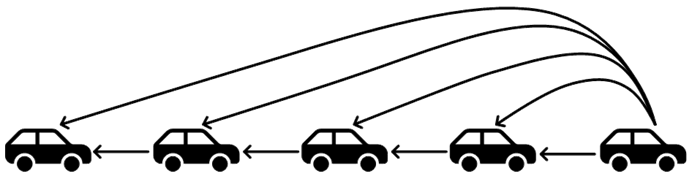
\includegraphics[width=8.5cm]{figs/fig1.png}
  \caption{~The schematic of the CAV platoon with Predecessor-Leader-Follower (PLF), the widely adopted IFT.}
  \label{fig1}
\end{figure}

Consider a group of n CAVs moving along a single lane organizing as a CAV platoon where the intra-vehicle communication functions according to the IFT. Fig.~\ref{fig1} shows the schematic of the CAV platoon with Predecessor-Leader-Follower (PLF), the widely adopted IFT. Via intra-vehicle communication (e.g., C-V2X, according to the meeting report from Federal Communications Commission \citep{POPEO2020}), all vehicles share their state information (e.g., the absolute position, the velocity, and the acceleration) with their neighbors according to the IFT. It is assumed that each CAV is equipped with i) an onboard radar responsible for collision detection via measuring the gap distance between any two consecutive vehicles, ii) a built-in GPS sensor for measuring the vehicular longitudinal position information, iii) a wireless onboard unit for communicating information of interest with its proximal vehicles via the C-V2X communication \citep{Mannoni2019}, iv) an upper-level controller for calculating the desired longitudinal acceleration based on the parameters obtained, and v) an engine actuator for determining the throttle and brake actuator inputs to track the desired acceleration. Such an assumption is reasonable because the sensing, communication, and actuation units required above are available in modern CAVs and therefore do not require specific changes to the existing vehicle configuration. Note that the surrounding information obtained by onboard radar only functions as the validation data only in case of communication unavailability or failure, as more accurate information can be obtained faster through communication.

\subsection{Vehicle longitudinal dynamic Modeling}
\label{Section 3.1}

A vehicle longitudinal dynamic model mainly consists of the engine, throttle and brake actuators, drive train, transmission, and torque converter. Under a variety of resistance forces, the longitudinal dynamics of vehicle $i$ can be modeled by the following force balance equation:
\begin{equation}
  m_ia_i(t)=f_i^e(t)-f_i^g(t)-f_i^w(t)-f_i^r(t),
  \label{eq1}
\end{equation}
where $m_i$ stands for the unknown mass of vehicle $i$; $f_i^e(t)$ is the desired engine force acting on the vehicle $i$; $f_i^g(t)$,$\ f_i^w(t)$, and $f_i^r(t)$ denote the gravity component parallel to the road surface, air resistance force, and rolling resistance force, respectively.

From designing a control strategy, the nonlinear vehicle dynamic model~(\ref{eq1}) is obviously unsuitable due to its nonlinear characteristics. Fortunately, by adopting nonlinear state feedback in Appendix A, the engine dynamic can be transformed into a linearized model \citep{Wang2018e}:
\begin{equation}
  \tau_i\dot{a_i}\left(t\right)+a_i\left(t\right)=u_i(t-\phi_i),
  \label{eq2}
\end{equation}
where $u_i(t)$ denotes the control input of the engine actuator, which can be interpreted as the desired acceleration of vehicle $i$; $\tau_i$ and $\phi_i$ are the time constants representing the engine actuator and internal communication delays.

We remark that the engine dynamic employed is Equation~(\ref{eq2}), based on field experimental data fitting, and differs from the first-order inertial time delay widely used in existing research \citep{Wang2018e,Coskun2021,Zhang2021,Ma2021}. Although supplementing in the main text can increase the effort of this paper. However, since this part is not very relevant to the main contribution of this paper, the specific experimental and fitting details are attached to Appendix B for the sake of simplicity.

Reformulate Equation~(\ref{eq2}), and the state space equation can be represented as:
\begin{equation}
  {\dot x_i}\left( t \right) = A{x_i}\left( t \right) + B{u_i}\left( {t - {\phi _i}} \right),
  \label{eq3}
\end{equation}
with
\begin{equation}
  A = \left[ {\begin{array}{*{20}{c}}
          0 & 1 & 0                          \\
          0 & 0 & 1                          \\
          0 & 0 & { - \frac{1}{{{\tau _i}}}}
        \end{array}} \right],B = \left[ {\begin{array}{*{20}{c}}
          0 \\
          0 \\
          {\frac{1}{{{\tau _i}}}}
        \end{array}} \right].
  \label{eq4}
\end{equation}
where ${x_i}\left( t \right) = {\left[ {\begin{array}{*{20}{c}}
          {{p_i}\left( t \right)} & {{v_i}\left( t \right)} & {{a_i}\left( t \right)}
        \end{array}} \right]^T} \in {\mathbb{R}^3}$ denotes the state vector of vehicle $i$.

Subject to limited communication, the inputs for vehicle $i$ are controlled by an appropriate decentralized coupling protocol of communication information:
\begin{equation}
  {u_i}\left( t \right) = {u_i}\underbrace {\left( {{x_1}\left( {t - h} \right), \cdots ,{x_i}\left( t \right), \cdots ,{x_n}\left( {t - h} \right)} \right)}_n,
  \label{eq6}
\end{equation}
where $h$ represents the communication delay within the transmission range which is assumed to be identical among the IFT \citep{Razzaghpour2022,Sehla2022,Vukadinovic2018a,Vu2020a,Martin-Sacristan2020a}.

Here we assume that CAVs adopt the Constant Time Headway (CTH) policy in which CAVs maintain a desired time headway from the reference vehicle. Then the cooperative tracking problem of vehicle $i$ can be formulated as:
\begin{equation}
  \left\{ \begin{gathered}
    \mathop {\lim }\limits_{t \to \infty } \left\| {\sum\limits_{j = 1}^n {\left| {{p_i}(t) - {p_j}(t - h){\text{ + }}{h_{ij}}{v_i}(t)} \right|} } \right\| = 0, \hfill \\
    \mathop {\lim }\limits_{t \to \infty } \left\| {\sum\limits_{j = 1}^n {\left| {{v_i}(t) - {v_j}(t - h)} \right|} } \right\| = 0, \hfill \\
    \mathop {\lim }\limits_{t \to \infty } \left\| {\sum\limits_{j = 1}^n {\left| {{a_i}(t) - {a_j}(t - h)} \right|} } \right\| = 0, \hfill \\
  \end{gathered}  \right.\forall i = 1, \ldots ,N,
  \label{eq7}
\end{equation}
where ${h_{ij}} =  - {h_{ji}}$ stands for the constant time headway between vehicle $i$ and vehicle $j$.

The consensus goal~(\ref{eq7}) can be achieved using an appropriate distributed control strategy. Therefore, the vehicle $i$ adjusts its dynamics through the following decentralized coupling protocol computed onboard:
\begin{equation}
  {u_i} =  - \sum\limits_{j = 1}^n {{a_{ij}}{k_{ij}}^T{{\left[ {\begin{array}{*{20}{c}}
              {{p_i}\left( t \right) - {p_j}\left( {t - h} \right) + {h_{ij}}{v_i}\left( t \right)}\\ {{v_i}\left( t \right) - {v_j}\left( {t - h} \right)}\\ {{a_i}\left( t \right) - {a_j}\left( {t - h} \right)}
            \end{array}} \right]}^T}},
  \label{eq8}
\end{equation}
where $a_{ij}$ denotes the weight of the edge $\left(i,j\right)$ and $a_{ij}=0$ if there is no edge $\left(i,j\right)$; $k_{ij}=\left[\begin{matrix}\alpha_{ij}&\beta_{ij}&\gamma_{ij}\\\end{matrix}\right]^T\in\mathbb{R}^{3\times1}$ presents the feedback control gain vector, with $\alpha_{ij}$, $\beta_{ij}$, and $\gamma_{ij}$ denote the control gain of spacing, speed, and acceleration errors.

\subsection{CAV platoon Modeling}
\label{Section 3.2}

To prove the consensus of systems~(\ref{eq3}) and~(\ref{eq6}) under the action of coupling protocol~(\ref{eq8}), the decentralized coupling protocol~(\ref{eq8}) can be reformulated as:
\begin{equation}
  {u_i} =  - \sum\limits_{j = 1}^n {{a_{ij}}{k_{ij}}^T\left[ {{\psi _{ij}}{x_i}(t) - {x_j}(t - h)} \right]} ,
  \label{eq10}
\end{equation}
where ${\psi _{ij}}{\text{ = }}\left[ {\begin{array}{*{20}{c}}
          1  & {{h_{ij}}} & {} \\
          {} & 1          & {} \\
          {} & {}         & 1
        \end{array}} \right]$ denotes the relationship between the states based on the CTH policy.

Therefore, the dynamics of the error system can be presented as follows:
\begin{equation}
  \left\{ \begin{gathered}
    {{\dot {\tilde p}}_i} = {{\tilde v}_i}, \hfill \\
    {{\dot {\tilde v}}_i} = {{\tilde a}_i}, \hfill \\
    {{\dot {\tilde a}}_i} =  - \frac{1}{\tau }{{\tilde a}_i} - \frac{1}{\tau }\sum\limits_{j = 0}^n {{a_{ij}}{k_{ij}}^T\left( {{\psi _{ij}}{x_i}(t - {\phi _i}) - {x_j}(t - {\phi _i}^*)} \right)},  \hfill \\
  \end{gathered}  \right.
  \label{eq11}
\end{equation}
where ${\phi_i}^\ast=\phi_i+h$.

From Equation~(\ref{eq11}), the dynamics of the closed-loop vehicular network can be recast in a compact form as:
\begin{equation}
  {\dot x_i}\left( t \right) = A{x_i}\left( t \right) - B\sum\limits_{j = 0}^n {{a_{ij}}{k_{ij}}^T\left( {{\psi _{ij}}{x_i}(t - {\phi _i}) - {x_j}(t - {\phi _i}^*)} \right)}.
  \label{eq12}
\end{equation}

\begin{theorem}
  The CAV platoon under CTH policy with multiple time delays can be modeled as a linear time-invariant state delay system:
  \begin{equation}
    \left\{ \begin{gathered}
      \dot X\left( t \right) = \Psi X\left( t \right) + {\Psi _{d1}}X(t - \phi ) + {\Psi _{d2}}X(t - {\phi ^*}),\quad \forall t \geqslant 0 \hfill \\
      X\left( t \right) = \varphi \left( t \right),\quad \quad \quad \quad \quad \quad \quad \forall t \in \left[ { - {\phi ^*},0} \right] \hfill \\
    \end{gathered}  \right.
    \label{eq13}
  \end{equation}
  with
  \begin{equation}
    \left\{ {\begin{array}{*{20}{l}}
          {\Psi  = {A^*} \in {\mathbb{R}^{3n \times 3n}}}                                                                                                                                     \\
          {{\Psi _{d1}} =  - {B^*}\mathcal{F}{E_1} \in {\mathbb{R}^{3n \times 3n}}{\text{ }}}                                                                                                 \\
          {{\Psi _{d2}} = {B^*}\mathcal{J}{E_2} \in {\mathbb{R}^{3n \times 3n}}{\text{ }}}                                                                                                    \\
          {{A^*} = {I_n} \otimes A \in {\mathbb{R}^{3n \times 3n}}}                                                                                                                           \\
          {{B^*} = {I_n} \otimes B \in {\mathbb{R}^{3n \times n}}}                                                                                                                            \\
          {\mathcal{K} = {{[{k_{ij}}^T]}_{n \times n}}{\text{ }}}                                                                                                                             \\
          {\mathcal{H} = {\mathcal{A} \circ }\mathcal{K} = {{[{a_{ij}} \otimes {k_{ij}}^T]}_{N \times N}} \in {\mathbb{R}^{n \times 3n}}{\text{ }}}                                           \\
          {\mathcal{J} = diag\underbrace {\left\{ {{\mathcal{D}_1},{\mathcal{D}_2}, \cdots ,{\mathcal{D}_N}} \right\}}_n \in {\mathbb{R}^{n \times 3{n^2}}}{\text{ }}}                        \\
          {\mathcal{F} = diag\underbrace {\left\{ {{\mathcal{H}_1},{\mathcal{H}_2}, \cdots ,{\mathcal{H}_N}} \right\}}_n \in {\mathbb{R}^{n \times 3{n^2}}}{\text{ }}}                        \\
          {{\mathcal{H}_i} = {\mathcal{D}_i} \circ \underbrace {\left[ {{\psi _{i1}},{\psi _{i2}}, \cdots ,{\psi _{in}}} \right]}_n \in {\mathbb{R}^{1 \times 3n}},\forall i \in \mathcal{V}} \\
          {{\mathcal{D}_i} = \underbrace {\left[ {{a_{i1}}{k_{i1}}^T,{a_{i2}}{k_{i2}}^T, \cdots ,{a_{in}}{k_{in}}^T} \right]}_n \in {\mathbb{R}^{1 \times 3n}},\forall i \in \mathcal{V}}     \\
          {{E_1} = diag\underbrace {\left\{ {{I_1},{I_1}, \cdots ,{I_1}} \right\}}_n \in {\mathbb{R}^{3{n^2} \times 3n}}}                                                                     \\
          {{E_2} = {{\underbrace {\left[ {\begin{array}{*{20}{c}}
                            {{I_2}^T} & \cdots & {{I_2}^T}
                          \end{array}} \right]}_n}^T} \in {\mathbb{R}^{3{n^2} \times 3n}}}                                                                     \\
          {{I_1} = {{\underbrace {\left[ {\begin{array}{*{20}{c}}
                            {{I_3}^T} & \cdots & {{I_3}^T}
                          \end{array}} \right]}_n}^T} \in {\mathbb{R}^{3n \times 3}}}                                                                          \\
          {{I_2} = {I_{3n}} \in {\mathbb{R}^{3n \times 3n}}}                                                                                                                                  \\
          {{I_3} = {I_3} \in {\mathbb{R}^{3 \times 3}}}
        \end{array}} \right.
  \end{equation}
  where $X\left(t\right)=\left[\begin{matrix}{x_1}^T&\cdots&{x_n}^T\\\end{matrix}\right]^T\in\mathbb{R}^{3n\times1}$ stands for the error state vector of the closed-loop vehicular network, $\varphi\left(t\right)$ is the initial condition, $\mathrm{\Psi}$,$\mathrm{\Psi}_{d1}$, and $\mathrm{\Psi}_{d2}$ are constant matrices according to their definitions.

  \label{theorem3}
\end{theorem}

\begin{proof}
  Theorem~\ref{theorem3} can be obtained by manipulating matrix transformations on the error state vector of the closed-loop vehicular network and Equation~(\ref{eq12}).
\end{proof}



% \citep{POPEO2020}
% \citep{Mannoni2019}
% \citep{Wang2018e,Coskun2021,Zhang2021,Ma2021}
% \citep{Razzaghpour2022,Sehla2022,Vukadinovic2018a,Vu2020a,Martin-Sacristan2020a}
% \begin{figure}
%   \centering

%   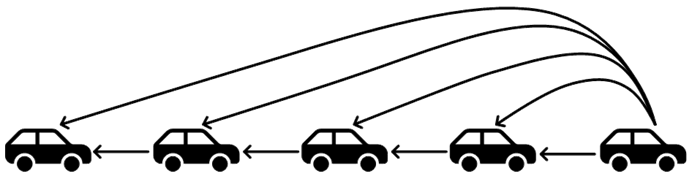
\includegraphics[width=14cm]{figs/fig1.png}
%   \caption{~.}
%   \label{fig1}
% \end{figure}



\section{Stability analyses}
\label{Section 4}
Before giving the stability criterion, we first introduce the Newton-Leibnitz formula, which is widely accepted:
\begin{equation}
  X(t - \phi ) = X(t) - \int_{t - \phi }^t {\dot X(s)ds}.
  \label{eq41}
\end{equation}

The primary idea of Lemma~\ref{lemma1} is to determine a positive definite functional whose derivative with respect to time along the trajectories of the system~(\ref{eq13}) is negative definite. Given the state delay system in Theorem~\ref{theorem3}~(\ref{eq13}), the delay-dependent stability criterion considering the relationship between $\phi$ and $\phi^\ast$ is established by employing Lemma~\ref{lemma1} according to the following Theorem.

\begin{theorem}
  Suppose a state-delay system~(\ref{eq13}) with two delays. The system is asymptotically stable if there exist matrices $P,Q_i,W_j,A_{jj},B_{jj},C_{jj}\in\mathbb{S}_n^+ with i=1,2,j=1,2,3$ and $n$ order matrices $N_i,S_i,M_i,A_{ij},B_{ij},C_{ij}$ with $i=1,2,3,i<j\le3$ such that the following LMIs holds:

  \begin{equation}
    \Theta  = \left[ {\begin{array}{*{20}{c}}
            {{\Theta _{11}} + {\Psi ^T}H\Psi } & {{\Theta _{12}} + {\Psi ^T}H{\Psi _{d1}}}    & {{\Theta _{13}} + {\Psi ^T}H{\Psi _{d2}}}    \\
            *                                  & {{\Theta _{22}} + \Psi _{d1}^TH{\Psi _{d1}}} & {{\Theta _{23}} + \Psi _{d1}^TH{\Psi _{d2}}} \\
            *                                  & *                                            & {{\Theta _{33}} + \Psi _{d2}^TH{\Psi _{d2}}}
          \end{array}} \right] \prec 0
    \label{eq42}
  \end{equation}
  \begin{equation}
    {\Xi _1} = \left[ {\begin{array}{*{20}{c}}
            {{A_{11}}} & {{A_{12}}} & {{A_{13}}} & {{N_1}} \\
            *          & {{A_{22}}} & {{A_{23}}} & {{N_2}} \\
            *          & *          & {{A_{33}}} & {{N_3}} \\
            *          & *          & *          & {{W_1}}
          \end{array}} \right] \succ 0
    \label{eq43}
  \end{equation}
  \begin{equation}
    {\Xi _2} = \left[ {\begin{array}{*{20}{c}}
            {{B_{11}}} & {{B_{12}}} & {{B_{13}}} & {{S_1}} \\
            *          & {{B_{22}}} & {{B_{23}}} & {{S_2}} \\
            *          & *          & {{B_{33}}} & {{S_3}} \\
            *          & *          & *          & {{W_2}}
          \end{array}} \right] \succ 0,
    \label{eq44}
  \end{equation}
  \begin{equation}
    {\Xi _3} = \left[ {\begin{array}{*{20}{c}}
            {{C_{11}}} & {{C_{12}}} & {{C_{13}}} & { - {M_1}} \\
            *          & {{C_{22}}} & {{C_{23}}} & { - {M_2}} \\
            *          & *          & {{C_{33}}} & { - {M_3}} \\
            *          & *          & *          & {{W_3}}
          \end{array}} \right] \succ 0,
    \label{eq45}
  \end{equation}

  where
  \begin{equation*}
    \begin{gathered}
      {\Theta _{11}} = P\Psi  + {\Psi ^T}P + {Q_1} + {Q_2} + {N_1} + N_1^{T} + {S_1} + S_1^{T} + \phi {A_{11}},\hfill \\
    \quad \quad + {\phi ^*}{B_{11}} + h{C_{11}}, \hfill \\
      {\Theta _{12}} = P{\Psi _{d1}} - {N_1} + N_2^{T} + S_2^{T} - {M_1} + \phi {A_{12}} + {\phi ^*}{B_{12}} + h{C_{12}}, \hfill \\
      {\Theta _{13}} = P{\Psi _{d2}} + N_3^{T} + S_3^{T} - {S_1} + {M_1} + \phi {A_{13}} + {\phi ^*}{B_{13}} + h{C_{13}}, \hfill \\
      {\Theta _{22}} =  - {Q_1} - {N_2} - N_2^{T} - {M_2} - M_2^{T} + \phi {A_{22}} + {\phi ^*}{B_{22}} + h{C_{22}}, \hfill \\
      {\Theta _{23}} =  - N_3^{T} - {S_2} + {M_2} - M_3^{T} + \phi {A_{23}} + {\phi ^*}{B_{23}} + h{C_{23}}, \hfill \\
      {\Theta _{33}} =  - {Q_2} - {S_3} - S_3^{T} + {M_3} + M_3^{T} + \phi {A_{33}} + {\phi ^*}{B_{33}} + h{C_{33}}, \hfill \\
      H = \phi {W_1} + {\phi ^*}{W_2} + h{W_3}. \hfill \\
    \end{gathered}
  \end{equation*}
  \label{theorem4}
\end{theorem}

\begin{proof}
  We first construct the LKF candidate as:
  \begin{equation}
    \begin{aligned}
      &V\left( {{X_t}} \right) =  {X^{T}}(t)PX(t) + \int_{t - \phi }^t {{X^{T}}} (s){Q_1}X(s){\text{d}}s \\
      &+ \int_{t - {\phi ^*}}^t {{X^{T}}} (s){Q_2}X(s){\text{d}}s  + \int_{ - \phi }^0 {\int_{t + \theta }^t {{{\dot X}^{T}}} } (s){W_1}\dot X(s){\text{d}}s\;{\text{d}}\theta  \\
      &+ \int_{ - {\phi ^*}}^0 {\int_{t + \theta }^t {{{\dot X}^{T}}} } (s){W_2}\dot X(s){\text{d}}s\;{\text{d}}\theta + \int_{ - {\phi ^*}}^{ - \phi } {\int_{t + \theta }^t {{{\dot X}^{T}}} } (s){W_3}\dot X(s){\text{d}}s\;{\text{d}}\theta. 
    \end{aligned}
    \label{eq46}
  \end{equation}
  where $P,Q_i,W_j\in\mathbb{S}_n^+$ with $i=1,2,j=1,2,3$ are to be determined.

  The positivity of the LKF candidate $V\left(X_t\right)$~(\ref{eq46}) is ensured by $P\succ0$,$Q_i\succ0$, and $W_j\succ0$ with $i=1,2,j=1,2,3$. Then another one that needs to be proven is the negativity of its derivative. Differentiating the functional~(\ref{eq46}) along the trajectories of the system~(\ref{eq13}) and replacing the $\dot{X}(t)$ in the first term yields:
  \begin{equation}
    \begin{aligned}
      \dot V\left( {{X_t}} \right) = & 2{X^{T}}(t)P\left[ {\Psi X(t) + {\Psi _{d1}}X\left( {t - \phi } \right) + {\Psi _{d2}}X\left( {t - {\phi ^*}} \right)} \right] \hfill \\
                                     & + {X^{T}}(t){Q_1}X(t) - {X^{T}}\left( {t - \phi } \right){Q_1}X\left( {t - \phi } \right) \hfill                                      \\
                                     & + {X^{T}}(t){Q_2}X(t) - {X^{T}}\left( {t - {\phi ^*}} \right){Q_2}X\left( {t - {\phi ^*}} \right) \hfill                              \\
                                     & + \phi {{\dot X}^{T}}(t){W_1}\dot X(t) - \int_{t - \phi }^t {{{\dot X}^{T}}} (s){W_1}\dot X(s){\text{d}}s \hfill                      \\
                                     & + {\phi ^*}{{\dot X}^{T}}(t){W_2}\dot X(t) - \int_{t - {\phi ^*}}^t {{{\dot X}^{T}}} (s){W_2}\dot X(s){\text{d}}s \hfill              \\
                                     & + h{{\dot X}^{T}}(t){W_3}\dot X(t) - \int_{t - {\phi ^*}}^{t - \phi } {{{\dot X}^{T}}} (s){W_3}\dot X(s){\text{d}}s. \hfill           \\
    \end{aligned}
    \label{eq47}
  \end{equation}

  Note that proving the negativity of $\dot{V}\left(X_t\right)$ directly is very difficult. Therefore, additional auxiliary equations based on the Newton-Leibnitz formula~(\ref{eq41}) are introduced:
  \begin{equation}
    \left\{ \begin{gathered}
      2\left[ {{X^{T}}(t){N_1} + } \right.\left. {{X^{T}}\left( {t - \phi } \right){N_2} + {X^{T}}\left( {t - {\phi ^*}} \right){N_3}} \right] \hfill \\
      \quad \quad \quad  \times \left[ {X(t) - X\left( {t - \phi } \right) - \int_{t - \phi }^t {\dot X} (s){\text{d}}s} \right] = 0, \hfill \\
      2\left[ {{X^{T}}(t){S_1} + } \right.\left. {{X^{T}}\left( {t - \phi } \right){S_2} + {X^{T}}\left( {t - {\phi ^*}} \right){S_3}} \right] \hfill \\
      \quad \quad \quad  \times \left[ {X(t) - X\left( {t - {\phi ^*}} \right) - \int_{t - {\phi ^*}}^t {\dot X} (s){\text{d}}s} \right] = 0, \hfill \\
      2\left[ {{X^{T}}(t){M_1} + } \right.\left. {{X^{T}}\left( {t - \phi } \right){M_2} + {X^{T}}\left( {t - {\phi ^*}} \right){M_3}} \right] \hfill \\
      \quad \quad \quad  \times \left[ {X\left( {t - {\phi ^*}} \right) - X\left( {t - \phi } \right) + \int_{t - {\phi ^*}}^{t - \phi } {\dot X} (s){\text{d}}s} \right] = 0. \hfill \\
    \end{gathered}  \right.
    \label{eq48}
  \end{equation}

  Moreover, another auxiliary equation is also introduced to help reveal the relationship between different delayed states:

  \begin{equation}
    {\left[ {\begin{array}{*{20}{c}}
              {X(t)}                        \\
              {X\left( {t - \phi } \right)} \\
              {X\left( {t - {\phi ^*}} \right)}
            \end{array}} \right]^{T}}\left[ {\begin{array}{*{20}{c}}
            {{\Lambda _{11}}} & {{\Lambda _{12}}} & {{\Lambda _{13}}} \\
            *                 & {{\Lambda _{22}}} & {{\Lambda _{23}}} \\
            *                 & *                 & {{\Lambda _{33}}}
          \end{array}} \right]\left[ {\begin{array}{*{20}{c}}
            {X(t)}                        \\
            {X\left( {t - \phi } \right)} \\
            {X\left( {t - {\phi ^*}} \right)}
          \end{array}} \right] = 0,
    \label{eq49}
  \end{equation}
  where $\mathrm{\Lambda}_{ij}=\phi\left(A_{ij}-A_{ij}\right)+\phi^\ast\left(B_{ij}-B_{ij}\right)+h\left(C_{ij}-C_{ij}\right),i=1,2,3,i\le j\le 3$.

  Then adding Equations~(\ref{eq48}) and~(\ref{eq49}) to the right-hand side of $\dot{V}\left(X_t\right)$ leads to:
  \begin{equation}
    \begin{aligned}
    \dot V\left( {{X_t}} \right) =& \eta _1^{T}(t)\Theta {\eta _1}(t) - \int_{t - \phi }^t {\eta _2^{T}} (t,s){\Xi _1}{\eta _2}(t,s){\text{d}}s \\
    & - \int_{t - {\phi ^*}}^t {\eta _2^{T}} (t,s){\Xi _2}{\eta _2}(t,s){\text{d}}s - \int_{t - {\phi ^*}}^{t - \phi } {\eta _2^{T}} (t,s){\Xi _3}{\eta _2}(t,s){\text{d}}s
    \end{aligned}
    \label{eq410}
  \end{equation}
  where
  \begin{equation*}
    \begin{aligned}
       & {\eta _1}(t) = {\left[ {{X^{T}}(t),{X^{T}}\left( {t - \phi } \right),{X^{T}}\left( {t - {\phi ^*}} \right)} \right]^{T}},                     \\
       & {\eta _2}(t,s) = {\left[ {{X^{T}}(t),{X^{T}}\left( {t - \phi } \right),{X^{T}}\left( {t - {\phi ^*}} \right),{{\dot X}^{T}}(s)} \right]^{T}}.
    \end{aligned}
  \end{equation*}

  If $\mathrm{\Theta} \prec 0$ and $\mathrm{\Xi}_i\succ0$ with $i=1,2,3$, then $\dot{V}\left(X_t\right)<-\varsigma\left|X(t)\right|$ for a sufficiently $\varsigma>0$. Therefore, the system~(\ref{eq13}) is asymptotically stable if LMIs~(\ref{eq42}) -~(\ref{eq45}) hold.

  \textbf{This completes the proof.}

\end{proof}

\begin{remark}
  \label{remarkdiff}
  The primary idea of the Lyapunov-Krasovskii stability theorem is that it is not necessary to ensure the negative definiteness of $V\left(t,X\left(t\right)\right)$ along all the trajectories of the system. Indeed, it is sufficient to ensure its negative definiteness only for the solutions that tend to escape the neighborhood of $V\left(t,X\left(t\right)\right)\le c$ of the equilibrium. The specific theoretical analysis is conducted in detail in Appendix D.
\end{remark}

\begin{remark}
  The main modification to the LKF candidate $V\left(X_t\right)$ is the addition of the last term. It represents the integral of the states between the time delays $\phi$ and $\phi^\ast$. Thanks to this term, the lower bound of the stability range corresponding to each time delay is non-zero, thus deriving more accurate results.
\end{remark}

\begin{remark}
  Unlike the traditional method of constructing a fixed-weighting matrix for the first auxiliary equation set~(\ref{eq48}), the free-weighting matrix is applied here since it allows free-weight matrices instead of constant-weight matrices. The weighting-matrices $N_i,S_i,M_i$ with $i=1,2,3$ are free and obtained optimally by solving the LMIs, thus further deriving more accurate results.
\end{remark}

The stability criterion of the deterministic system can be obtained by Theorem~\ref{theorem4}. However, deterministic systems exist only under the ideal condition due to the existence of errors and disturbances in practice. Therefore, the robust stability criterion for systems with uncertainties must be explored. Suppose the state delay system~(\ref{eq13}) under time-varying structured uncertainties \citep{Shamma1994,Wu2021,Wu2004}, and it can be described by:
\begin{equation}
  \left\{ \begin{gathered}
    \dot X\left( t \right) = (\Psi  + \Delta \Psi (t))X\left( t \right) + ({\Psi _{d1}} + \Delta {\Psi _{d1}}(t))X(t - \phi ) \hfill \\
    \quad\quad + ({\Psi _{d2}} + \Delta {\Psi _{d2}}(t))X(t - {\phi ^*}),\quad \forall t \geqslant 0, \hfill \\
    X\left( t \right) = \varphi \left( t \right),\quad \quad \quad \quad \quad \quad \quad \forall t \in \left[ { - {\phi ^*},0} \right]. \hfill \\
  \end{gathered}  \right..
  \label{eq411}
\end{equation}

The uncertainties are assumed to be of the form:
\begin{equation}
  \left[ {\begin{array}{*{20}{c}}
          {\Delta \Psi (t)} & {\Delta {\Psi _{d1}}(t)} & {\Delta {\Psi _{d2}}(t)}
        \end{array}} \right] = DF(t)\left[ {\begin{array}{*{20}{c}}
          E & {{E_{d1}}} & {{E_{d2}}}
        \end{array}} \right],
  \label{eq4XX}
\end{equation}
where $D$, $E$, $E_{d1}$ and $E_{d2}$ are constant matrices with appropriate dimensions; and $F(t)$ is an unknown real-time-varying matrix with Lebesgue-measurable elements satisfying:
\begin{equation}
  {F^{\text{T}}}(t)F(t) \le I,  \forall t.
  \label{eq4XX2}
\end{equation}

Then, the stability criterion of the state delay system under time-varying structured uncertainties~(\ref{eq411}) is established by employing the Lemma~\ref{lemmaX1} and Lemma~\ref{lemmaX2} according to the following Theorem.

\begin{theorem}
  Suppose a state-delay system under time-varying structured uncertainties~(\ref{eq411}) with two delays. The system is robustly stable if there exist matrices $P,Q_i,W_j,A_{jj},B_{jj},C_{jj}\in\mathbb{S}_n^+$ with $i=1,2,j=1,2,3$,$n$ order matrices $N_i,S_i,M_i,A_{ij},B_{ij},C_{ij}$ with $i=1,2,3,i<j\le3$, and a scalar $\lambda>0$ such that LMIs~(\ref{eq43})-~(\ref{eq45}) and the following LMIs holds:
  \begin{equation}
    \left[ {\begin{array}{*{20}{c}}
            {{{\tilde \Theta }_{11}}} & {{{\tilde \Theta }_{12}}} & {{{\tilde \Theta }_{13}}} & {{\Psi ^T}H}    & {PD}           \\
            *                         & {{{\tilde \Theta }_{22}}} & {{{\tilde \Theta }_{23}}} & {\Psi _{d1}^TH} & 0              \\
            *                         & *                         & {{{\tilde \Theta }_{33}}} & {\Psi _{d2}^TH} & 0              \\
            *                         & *                         & *                         & { - H}          & {HD}           \\
            *                         & *                         & *                         & *               & { - \lambda I}
          \end{array}} \right] \prec 0,
    \label{eq412}
  \end{equation}
  where
  \begin{small}
  \begin{equation*}
    \begin{gathered}
      {{\tilde \Theta }_{11}} = P\Psi  + {\Psi ^T}P + {Q_1} + {Q_2} + {N_1} + N_1^{\text{T}} + {S_1} + S_1^{\text{T}} + \lambda {E^T}E + \phi {A_{11}},\hfill\\
       \quad \quad + {\phi ^*}{B_{11}} + h{C_{11}}, \hfill \\
      {{\tilde \Theta }_{12}} = P{\Psi _{d1}} - {N_1} + N_2^{\text{T}} + S_2^{\text{T}} - {M_1} + \lambda {E^T}{E_{d1}} + \phi {A_{12}} + {\phi ^*}{B_{12}} + h{C_{12}}, \hfill \\
      {{\tilde \Theta }_{13}} = P{\Psi _{d2}} + N_3^{\text{T}} + S_3^{\text{T}} - {S_1} + {M_1} + \lambda {E^T}{E_{d2}} + \phi {A_{13}} + {\phi ^*}{B_{13}} + h{C_{13}}, \hfill \\
      {{\tilde \Theta }_{22}} =  - {Q_1} - {N_2} - N_2^{\text{T}} - {M_2} - M_2^{\text{T}} + \lambda E_{d1}^T{E_{d1}} + \phi {A_{22}} + {\phi ^*}{B_{22}} + h{C_{22}}, \hfill \\
      {{\tilde \Theta }_{23}} =  - N_3^{\text{T}} - {S_2} + {M_2} - M_3^{\text{T}} + \lambda E_{d1}^T{E_{d2}} + \phi {A_{23}} + {\phi ^*}{B_{23}} + h{C_{23}}, \hfill \\
      {{\tilde \Theta }_{33}} =  - {Q_2} - {S_3} - S_3^{\text{T}} + {M_3} + M_3^{\text{T}} + \lambda E_{d2}^T{E_{d2}} + \phi {A_{33}} + {\phi ^*}{B_{33}} + h{C_{33}}. \hfill \\
    \end{gathered}
  \end{equation*}
\end{small}
  \label{theorem7}
\end{theorem}

\begin{proof}
  The proof of Theorem~\ref{theorem7} is similar to the proof of Theorem~\ref{theorem4}, differing only in the process of deriving LMI~(\ref{eq412}). Replacing $\mathrm{\Psi}$, $\mathrm{\Psi}_{d1}$, and $\mathrm{\Psi}_{d2}$ in Equation~(\ref{eq42}) with $\mathrm{\Psi}+DF(t)E$, $\mathrm{\Psi}_{d1}+DF(t)E_{d1}$, and $\mathrm{\Psi}_{d2}+DF(t)E_{d2}$, respectively. Then applying Schur complement to the LMI yields:
  \begin{equation}
    \begin{aligned}
    &\left[ {\begin{array}{*{20}{c}}
            {{\Theta _{11}}} & {{\Theta _{12}}} & {{\Theta _{13}}} & {{\Psi ^T}H}    \\
            *                & {{\Theta _{22}}} & {{\Theta _{23}}} & {\Psi _{d1}^TH} \\
            *                & *                & {{\Theta _{33}}} & {\Psi _{d2}^TH} \\
            *                & *                & *                & { - H}
          \end{array}} \right] \\&+ \left[ {\begin{array}{*{20}{c}}
            {PD} \\
            0    \\
            0    \\
            {HD}
          \end{array}} \right]F(t)\left[ {\begin{array}{*{20}{c}}
            E & {{E_{d1}}} & {{E_{d2}}} & 0
          \end{array}} \right] \\&+ \left[ {\begin{array}{*{20}{c}}
            {{E^T}}    \\
            {E_{d1}^T} \\
            {E_{d2}^T} \\
            0
          \end{array}} \right]{F^T}(t)\left[ {\begin{array}{*{20}{c}}
            {{D^T}{P^T}} & 0 & 0 & {{D^T}{H^T}}
          \end{array}} \right] \prec 0.
        \end{aligned}
    \label{eq413}
  \end{equation}

  According to Lemma~\ref{lemmaX1}, if there exists a scalar $\lambda>0$, then the LMI~(\ref{eq413}) is equivalent to the following LMI:
  \begin{equation}
    \begin{aligned}
    &\left[ {\begin{array}{*{20}{c}}
            {{\Theta _{11}}} & {{\Theta _{12}}} & {{\Theta _{13}}} & {{\Psi ^T}H}    \\
            *                & {{\Theta _{22}}} & {{\Theta _{23}}} & {\Psi _{d1}^TH} \\
            *                & *                & {{\Theta _{33}}} & {\Psi _{d2}^TH} \\
            *                & *                & *                & { - H}
          \end{array}} \right] \\
          &+ {\lambda ^{ - 1}}\left[ {\begin{array}{*{20}{c}}
            {PD} \\
            0    \\
            0    \\
            {HD}
          \end{array}} \right]\left[ {\begin{array}{*{20}{c}}
            {{D^T}{P^T}} & 0 & 0 & {{D^T}{H^T}}
          \end{array}} \right] \\
         & + \lambda \left[ {\begin{array}{*{20}{c}}
            {{E^T}}    \\
            {E_{d1}^T} \\
            {E_{d2}^T} \\
            0
          \end{array}} \right]\left[ {\begin{array}{*{20}{c}}
            E & {{E_{d1}}} & {{E_{d2}}} & 0
          \end{array}} \right] \prec 0.
        \end{aligned}
    \label{eq414}
  \end{equation}

  Applying the Schur complement to the LMI~(\ref{eq414}) yields LMI~(\ref{eq412}).

  \textbf{This completes the proof.}

\end{proof}

% \citep{Shamma1994,Wu2021,Wu2004}
\section{Numerical analyses}
\label{Section 5}
In this section, extensive numerical simulations and analyses on tracking performances and safety conditions of the CAV platoon employing the PLF illustrate the main results. Moreover, the tracking performances of the CAV platoon adopting different control parameters are also analyzed.

\subsection{Numerical Setup}
\label{Section 5.1}

To conduct comprehensive performance evaluation analyses, we choose a CAV platoon containing 5 CAVs interconnected by PLF, as shown in Fig.~\ref{fig1}. The Leader CAV drives under a given speed profile while the other CAVs drive under the control strategy. Note that the transfer function of the engine actuator considering the engine actuator and internal communication delays is as follows, which is obtained based on the experimental data introduced in detail in Appendix B:
\begin{equation}
  G_i(s)=\frac{k_G}{\tau_is+1}e^{-\phi_is}=\frac{1}{0.7148s+1}e^{-0.2s}
  \label{eq51}
\end{equation}

\begin{figure}

  \centering
  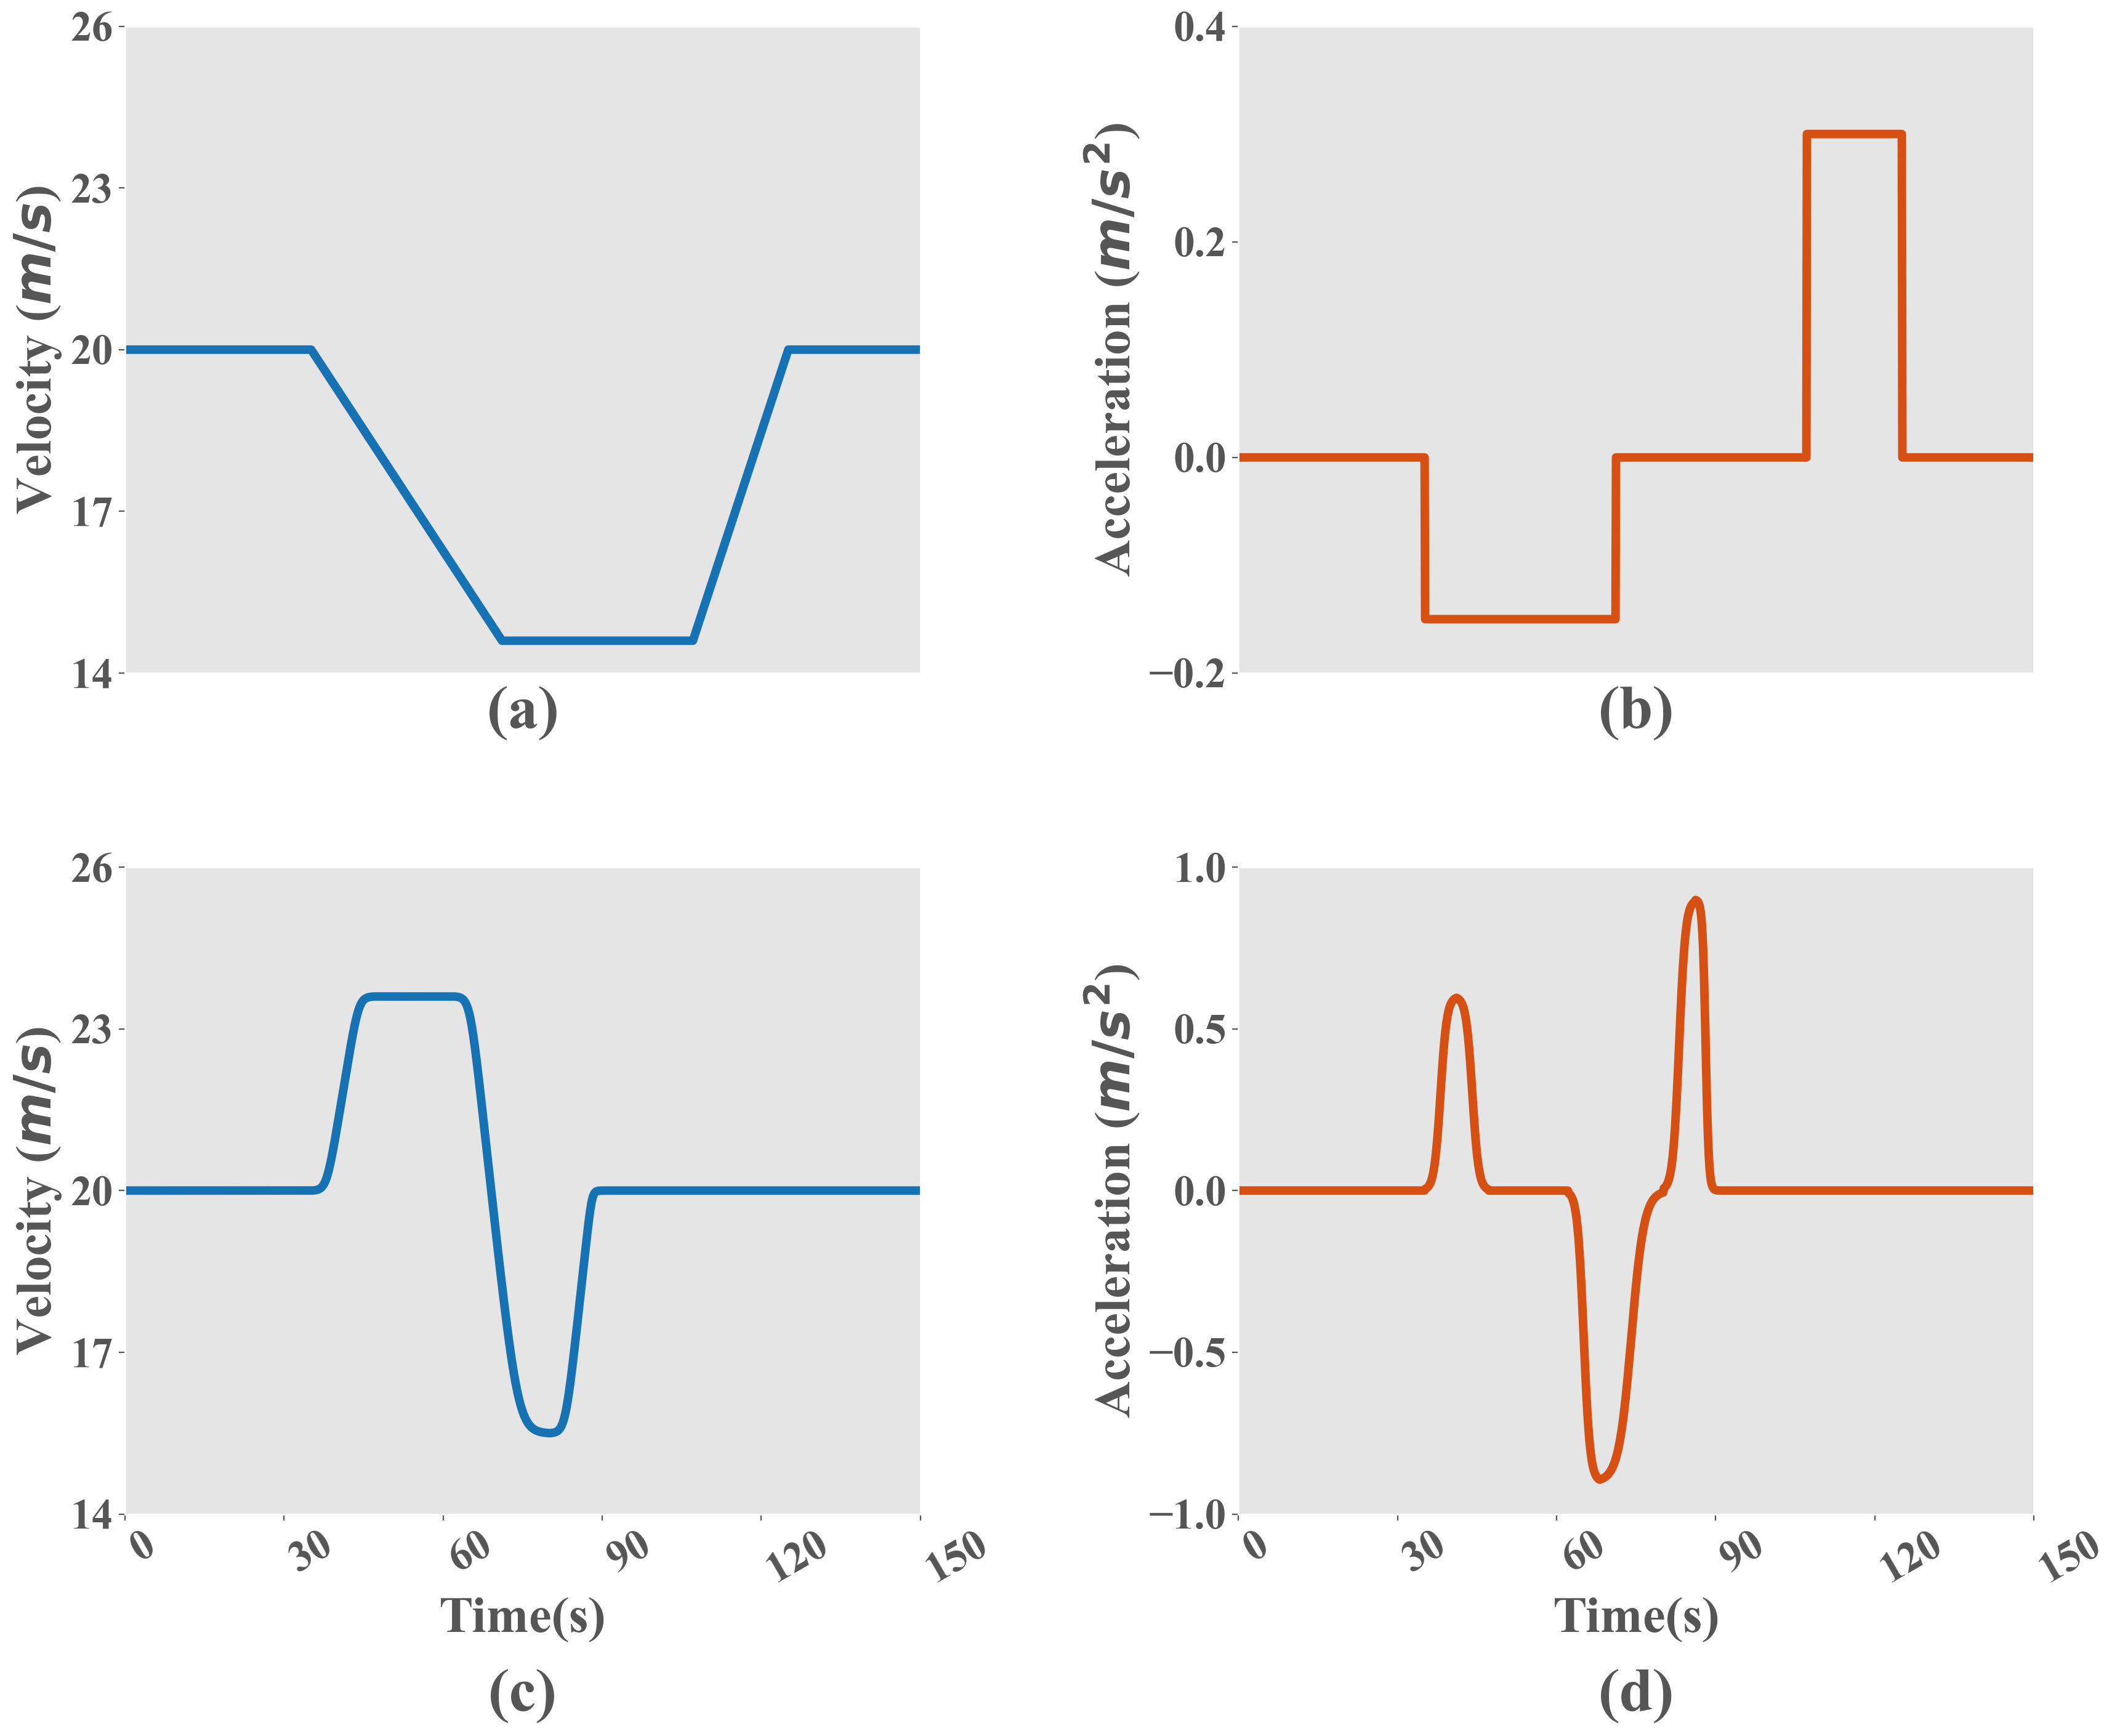
\includegraphics[width=8.5cm]{figs/fig2.png}
  \caption{~The two representative leader maneuvers: (a) and (b) denote the velocity and acceleration of the trapezoidal signal, respectively; (c) and (d) denote the velocity and acceleration of the oscillation signal, respectively.}
  \label{fig2}

\end{figure}

Moreover, parameters for both network and traffic simulation are set in Table~\ref{table1}, for simplicity but without loss of generality. In addition, to evaluate the tracking performances of the CAV platoon, two representative leader motions adopted in the simulation are depicted in Fig.~\ref{fig2} to simulate the response to perturbations transmitted from the upstream traffic flow:
\begin{enumerate}
  \item \textbf{Trapezoidal signal}: The leader suddenly decelerates to $14.6m/s$ at $ - 0.15m/{s^2}$ and keeps it for $36s$. Then the leader accelerates back to $20m/s$ at $ 0.3m/{s^2} $(see Fig.~\ref{fig2}(a, b)).
  \item \textbf{Oscillation signal}: The leader suddenly accelerates to $23.6m/s$ in $12s$ and keeps the velocity for $15s$. Then the leader decelerates to $16.4m/s$ in $12s$ and accelerates back to $20m/s$ in $12s$ (see Fig.~\ref{fig2}(c, d)).
\end{enumerate}

\begin{table}
  \centering
  \setlength{\abovecaptionskip}{0pt}
  \setlength{\belowcaptionskip}{10pt}%设置标题与表格的距离
  \begin{threeparttable}[b]
    \caption{~Network and traffic simulation parameters.}
    \label{table1}
    {\begin{tabular}{lc} \toprule
        Parameters                              & Value                \\ \midrule
        Platoon size $n$                        & 5 vehicles           \\
        Vehicle length $L$                      & 5 [m]                \\
        Engine actuator delay $\tau_i$          & 0.7148 [s]           \\
        Internal communication delay $\phi_{i}$ & 0.2 [s]              \\
        Communication delay $h$                 & 0.3 [s]    \tnote{1} \\
        \bottomrule
      \end{tabular}}
    \begin{tablenotes}
      \item[1] \citep{Vukadinovic2018a,Wang2018e}
    \end{tablenotes}
  \end{threeparttable}
\end{table}


\subsection{Numerical analyses of the CAV platoon considering internal communication delay and uncertainties}
\label{Section 5.2}

Within this subsection, the CAV platoon is targeted for analysis in which each CAV adopts the same control parameters satisfying Theorem~\ref{theorem4} and~\ref{theorem7}: $k_i=[0.3,0.3,0.3]^T$ and $h_i=0.6$. Furthermore, for investigating the impact of considering multiple delays and uncertainties on the tracking performances and safety conditions, detailed analyses are conducted on three cases, namely:
\begin{enumerate}

  \item \textit{Case \uppercase\expandafter{\romannumeral1}} Single delay: Only the engine actuator delay is considered, and the internal communication delay or the system uncertainty is ignored.
  \item \textit{Case \uppercase\expandafter{\romannumeral2}} Multiple delays: Where both the engine actuator and internal communication delays are considered, but the uncertainty of the system is ignored.
  \item \textit{Case \uppercase\expandafter{\romannumeral3}} Uncertain system: Here, both engine actuator and internal communication delays are considered, and system uncertainty is taken into account. For simulation, we consider the dynamic system uncertainties with the following setting so that the time-varying structured uncertainties function only on the measuring progress of the vehicle system:
        \begin{equation*}
          \left\{ \begin{aligned}
            & D=I, \\
            & F(t)=\sin t ,\\
            & E=I_n \otimes\left[\begin{array}{ccc}
            0 & 0.05 & 0 \\
            0 & 0 & 0.05 \\
            0 & 0 & 0.05
            \end{array}\right], \\
            & E_{d 1}=R_1 \otimes\left[\begin{array}{ccc}
            0 & 0 & 0 \\
            0 & 0 & 0 \\
            0.1 & 0.1 & 0.1
            \end{array}\right] \text {, } \\
            & E_{d 2}=R_2 \otimes\left[\begin{array}{ccc}
            0 & 0 & 0 \\
            0 & 0 & 0 \\
            0.07 & 0.07 & 0.07
            \end{array}\right], \\
            & R_1=\left[\begin{array}{lllll}
            0 & 0 & 0 & 0 & 0 \\
            1 & 0 & 0 & 0 & 0 \\
            0 & 1 & 0 & 0 & 0 \\
            0 & 0 & 1 & 0 & 0 \\
            0 & 0 & 0 & 1 & 0
            \end{array}\right], \\
            & R_2=\operatorname{diag}\{0,1,1,1,1\}. \\
            \end{aligned}
          \right.
        \end{equation*}
\end{enumerate}

Moreover, corresponding matrixes $P,Q_i,W_j,A_{ij},B_{ij},C_{ij}$ with $i=1,2,3,i<j\le3$ satisfying Theorem~\ref{theorem4} and~\ref{theorem7} can be found in Appendix E. A detailed analysis is carried out on the tracking performances and safety conditions.

% % \clearpage
\subsubsection{Tracking performance analyses}
\label{Section 5.2.1}

\begin{figure*}
  \centering
  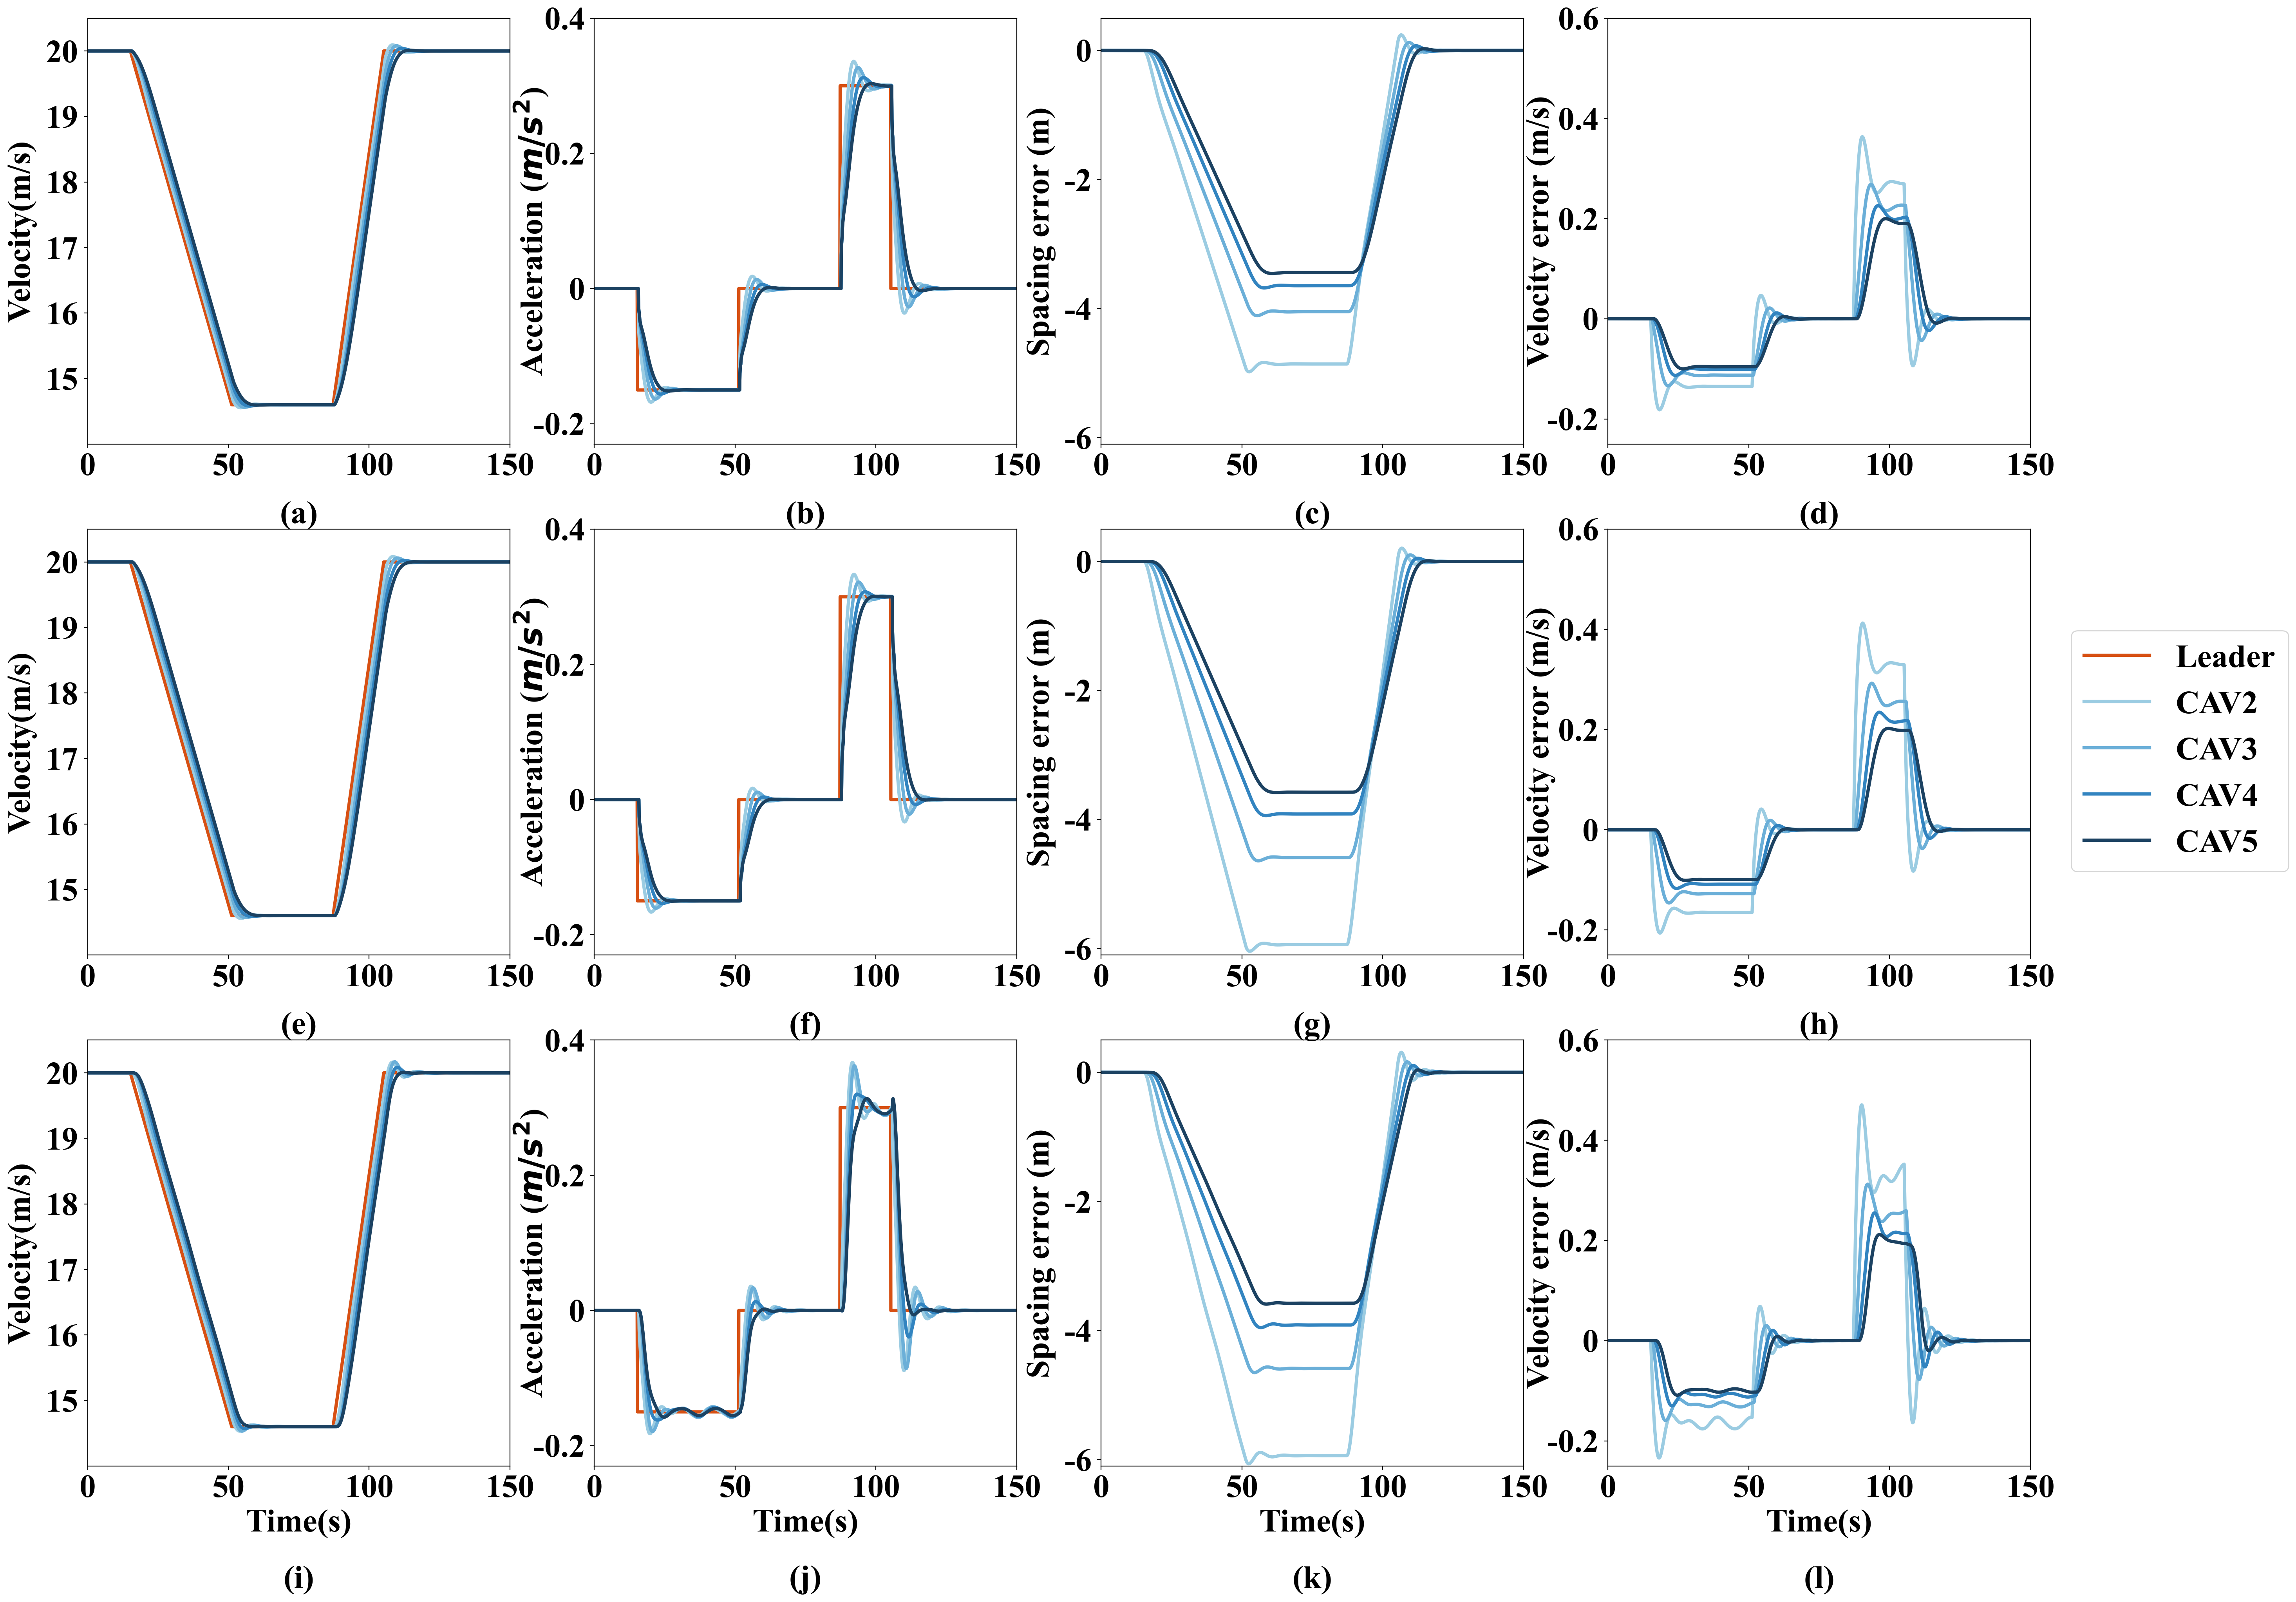
\includegraphics[width=16cm]{figs/fig3.png}
  \caption{~Tracking performances of the CAV platoon for the Trapezoidal signal in Fig. 2(a,b) under the three cases: (a), (b), (c), and (d) present tracking results under Case \uppercase\expandafter{\romannumeral1}, including the velocity, acceleration, tracking error of spacing, and tracking error of velocity, respectively; (e), (f), (g), and (h) show the case under Case  \uppercase\expandafter{\romannumeral2}; (i), (j), (k), and (l) denote the case under Case \uppercase\expandafter{\romannumeral3}.}
  \label{fig3}
\end{figure*}

After the CAV platoon has been composed and all CAVs have reached the equilibrium state, i.e., the tracking error is 0, the Trapezoidal signal is applied to the lead vehicle as shown in Fig.~\ref{fig2}(a,b), and then the corresponding tracking results are shown in Fig.~\ref{fig3}. This demonstrates that all CAVs are able to track the leader motion smoothly and revert to the equilibrium state, i.e., the steady-state error is zero, which means that the CAV platoon is stable in the simulation. Furthermore, the tracking errors of the tracking vehicle abruptly vary with the transients in the leader motion and then disappear over time. It should be noted that the transient response amplitude due to perturbation is significantly higher when considering internal communication delay compared to the case without considering. Indeed, this results from an untimely response caused by internal communication delay. As for the effect of uncertainties, the error fluctuation is more severe, and it takes longer to recover from the perturbation, although there is no significant difference in magnitude. In general, introducing the internal communication delay and uncertainties can cause poor tracking performance compared to the unconsidered case.

\begin{figure*}
  \centering
  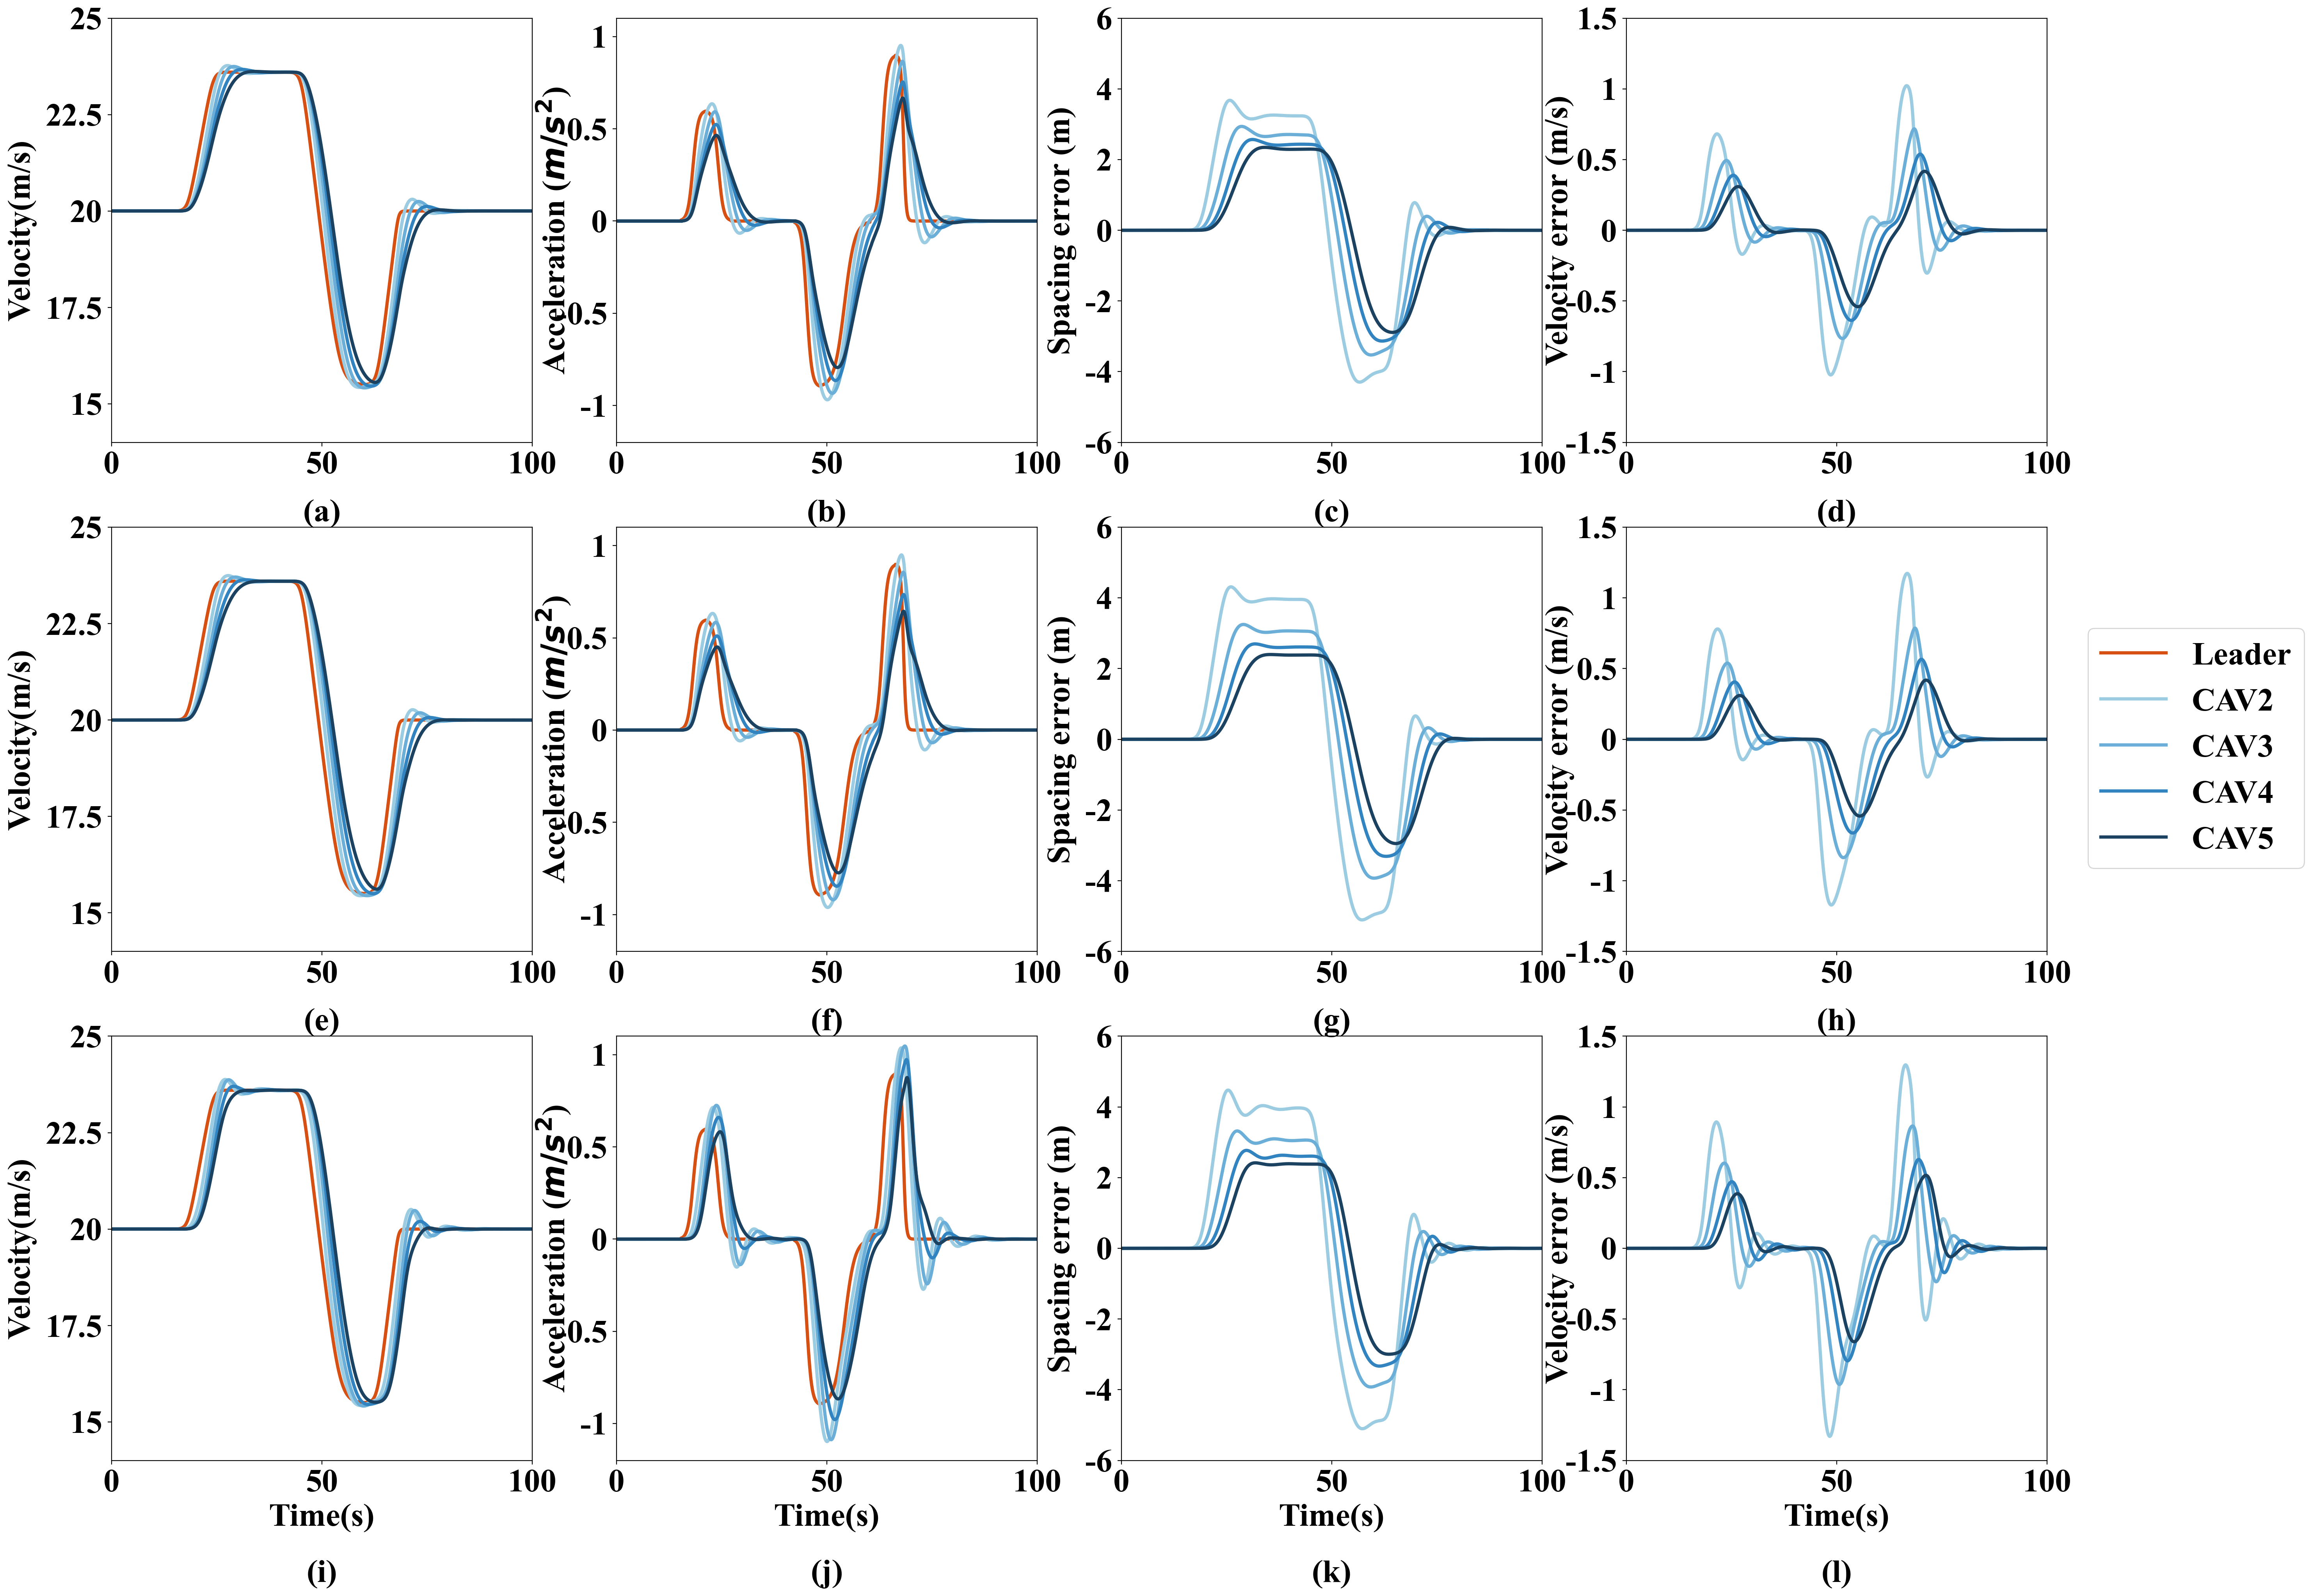
\includegraphics[width=16cm]{figs/fig4.png}
  \caption{~Tracking performances of the CAV platoon for the Oscillation signal in Fig. 2(c,d) under the three cases: (a), (b), (c), and (d) present tracking results under Case \uppercase\expandafter{\romannumeral1}, including the velocity, acceleration, tracking error of spacing, and tracking error of velocity, respectively; (e), (f), (g), and (h) show the case under Case  \uppercase\expandafter{\romannumeral2}; (i), (j), (k), and (l) denote the case under Case \uppercase\expandafter{\romannumeral3}.}
  \label{fig4}
\end{figure*}

Furthermore, the tracking performances of the three cases have also been adopted for the oscillation signal defined in Fig.~\ref{fig2}(c, d). The corresponding tracking performances of the three cases are illustrated in Fig.~\ref{fig4}. Under the oscillation signal, the cases under three cases still maintain excellent tracking performances, as shown in Fig.~\ref{fig4}, where each vehicle adjusts to changes in leader motion and returns to the equilibrium state with zero steady-state error. Besides, a similar phenomenon and conclusion can be obtained in Fig.~\ref{fig3} that introducing the internal communication delay and uncertainties deteriorates tracking performance.

To further investigate the specific impact of different cases on the transient response parallel to the stability, we selected two widely accepted indicators for evaluating transient response: Setting time (ST) and Maximum overshoot (MO). ST refers to "the time required for the response curve to reach and stay within a range of a certain percentage ($2\%$) of the final value". Moreover, MO refers to "the maximum peak value of the response curve measured from the desired response of the system" \citep{ogata1995discrete}. Among these two indicators, ST describes the time for the controller to recover from transient response to equilibrium, that is, the speed in the fundamental objective, while MO denotes the Maximum deviation caused by the transient response, which is another fundamental objective accuracy. By definition, smaller ST and MO indicate a better transient response, driving comfort, and safety. Also, since the investigation is on the differences in the transient response of different cases, the form of the leader motion has little effect on this, so the results are analyzed here only for the cases under the Trapezoidal signal.


\begin{figure*}
  \centering
  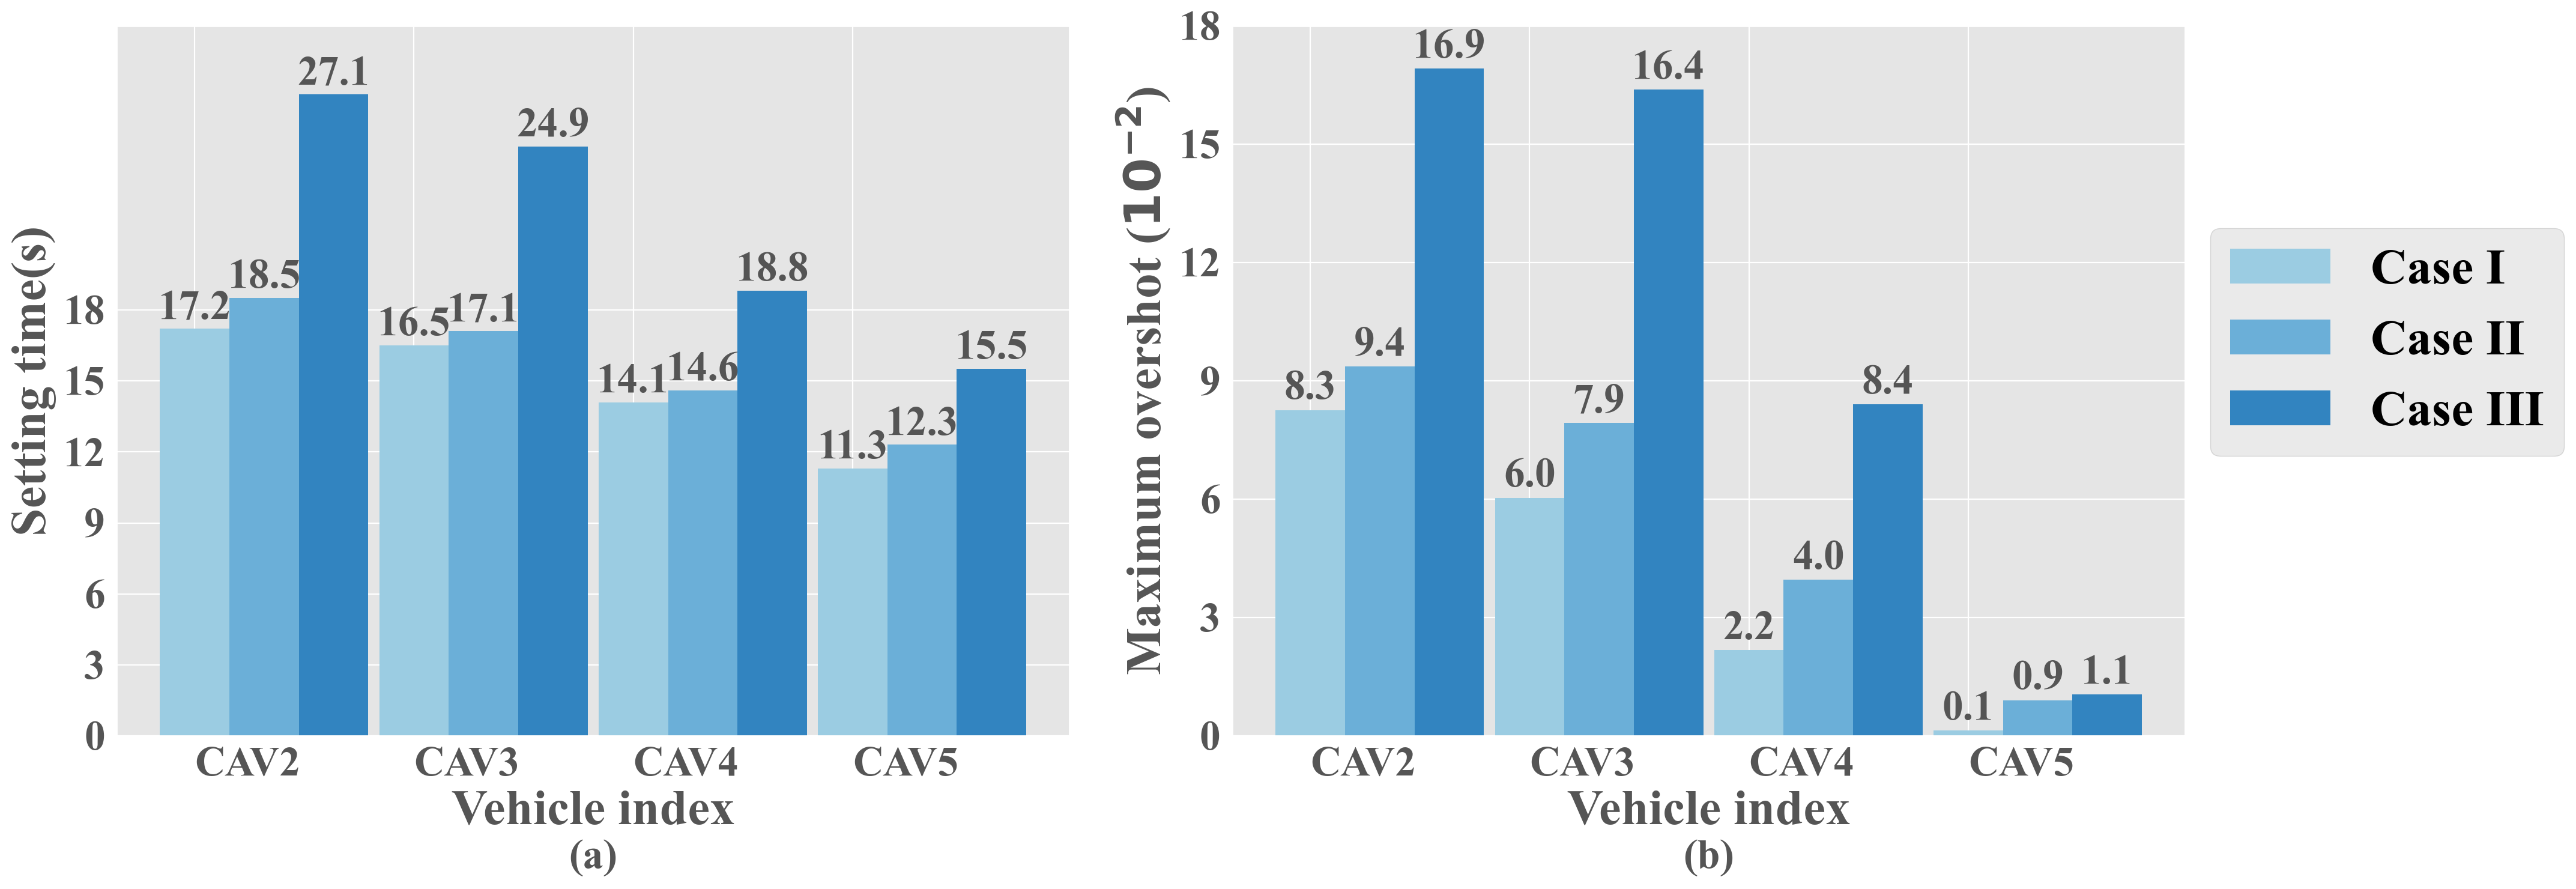
\includegraphics[width=16cm]{figs/fig5.png}
  \caption{~Indicators for evaluating the transient response of each CAV among the CAV platoon for the three cases: (a) the setting time; (b) the maximum overshoot.}
  \label{fig5}
\end{figure*}

Fig.~\ref{fig5} depicts the results of comparing three cases on the two indicators. On the one hand, considering internal communication delay and uncertainties lead to an increase in ST and MO, that is, a slower recovery to the equilibrium state and larger transient response amplitude. Specifically, the effect of internal communication delay is relatively minor, with only a $7.55\%$ increase in ST for CAV2, for example. However, the effect of uncertainties is significant, increasing the ST of CAV2 by $46.49\%$. Similar conclusions hold for MO. Therefore, considering uncertainties, a more realistic situation will have worse driving comfort and safety than the ideal situation. On the other hand, for all cases, both ST and MO decrease with the vehicle index increasing, indicating that the response amplitude excited by the perturbation decreases, and the recovery time from the perturbation to the equilibrium state becomes shorter, as the size of the CAV platoon increases. Indeed, these benefits of leader-based communication allow for more distant information to be obtained through leader-based communication and thus to react earlier to improve the transient response performance when the disturbance propagates with the size of the CAV platoon increasing.


\begin{figure}
  \centering
  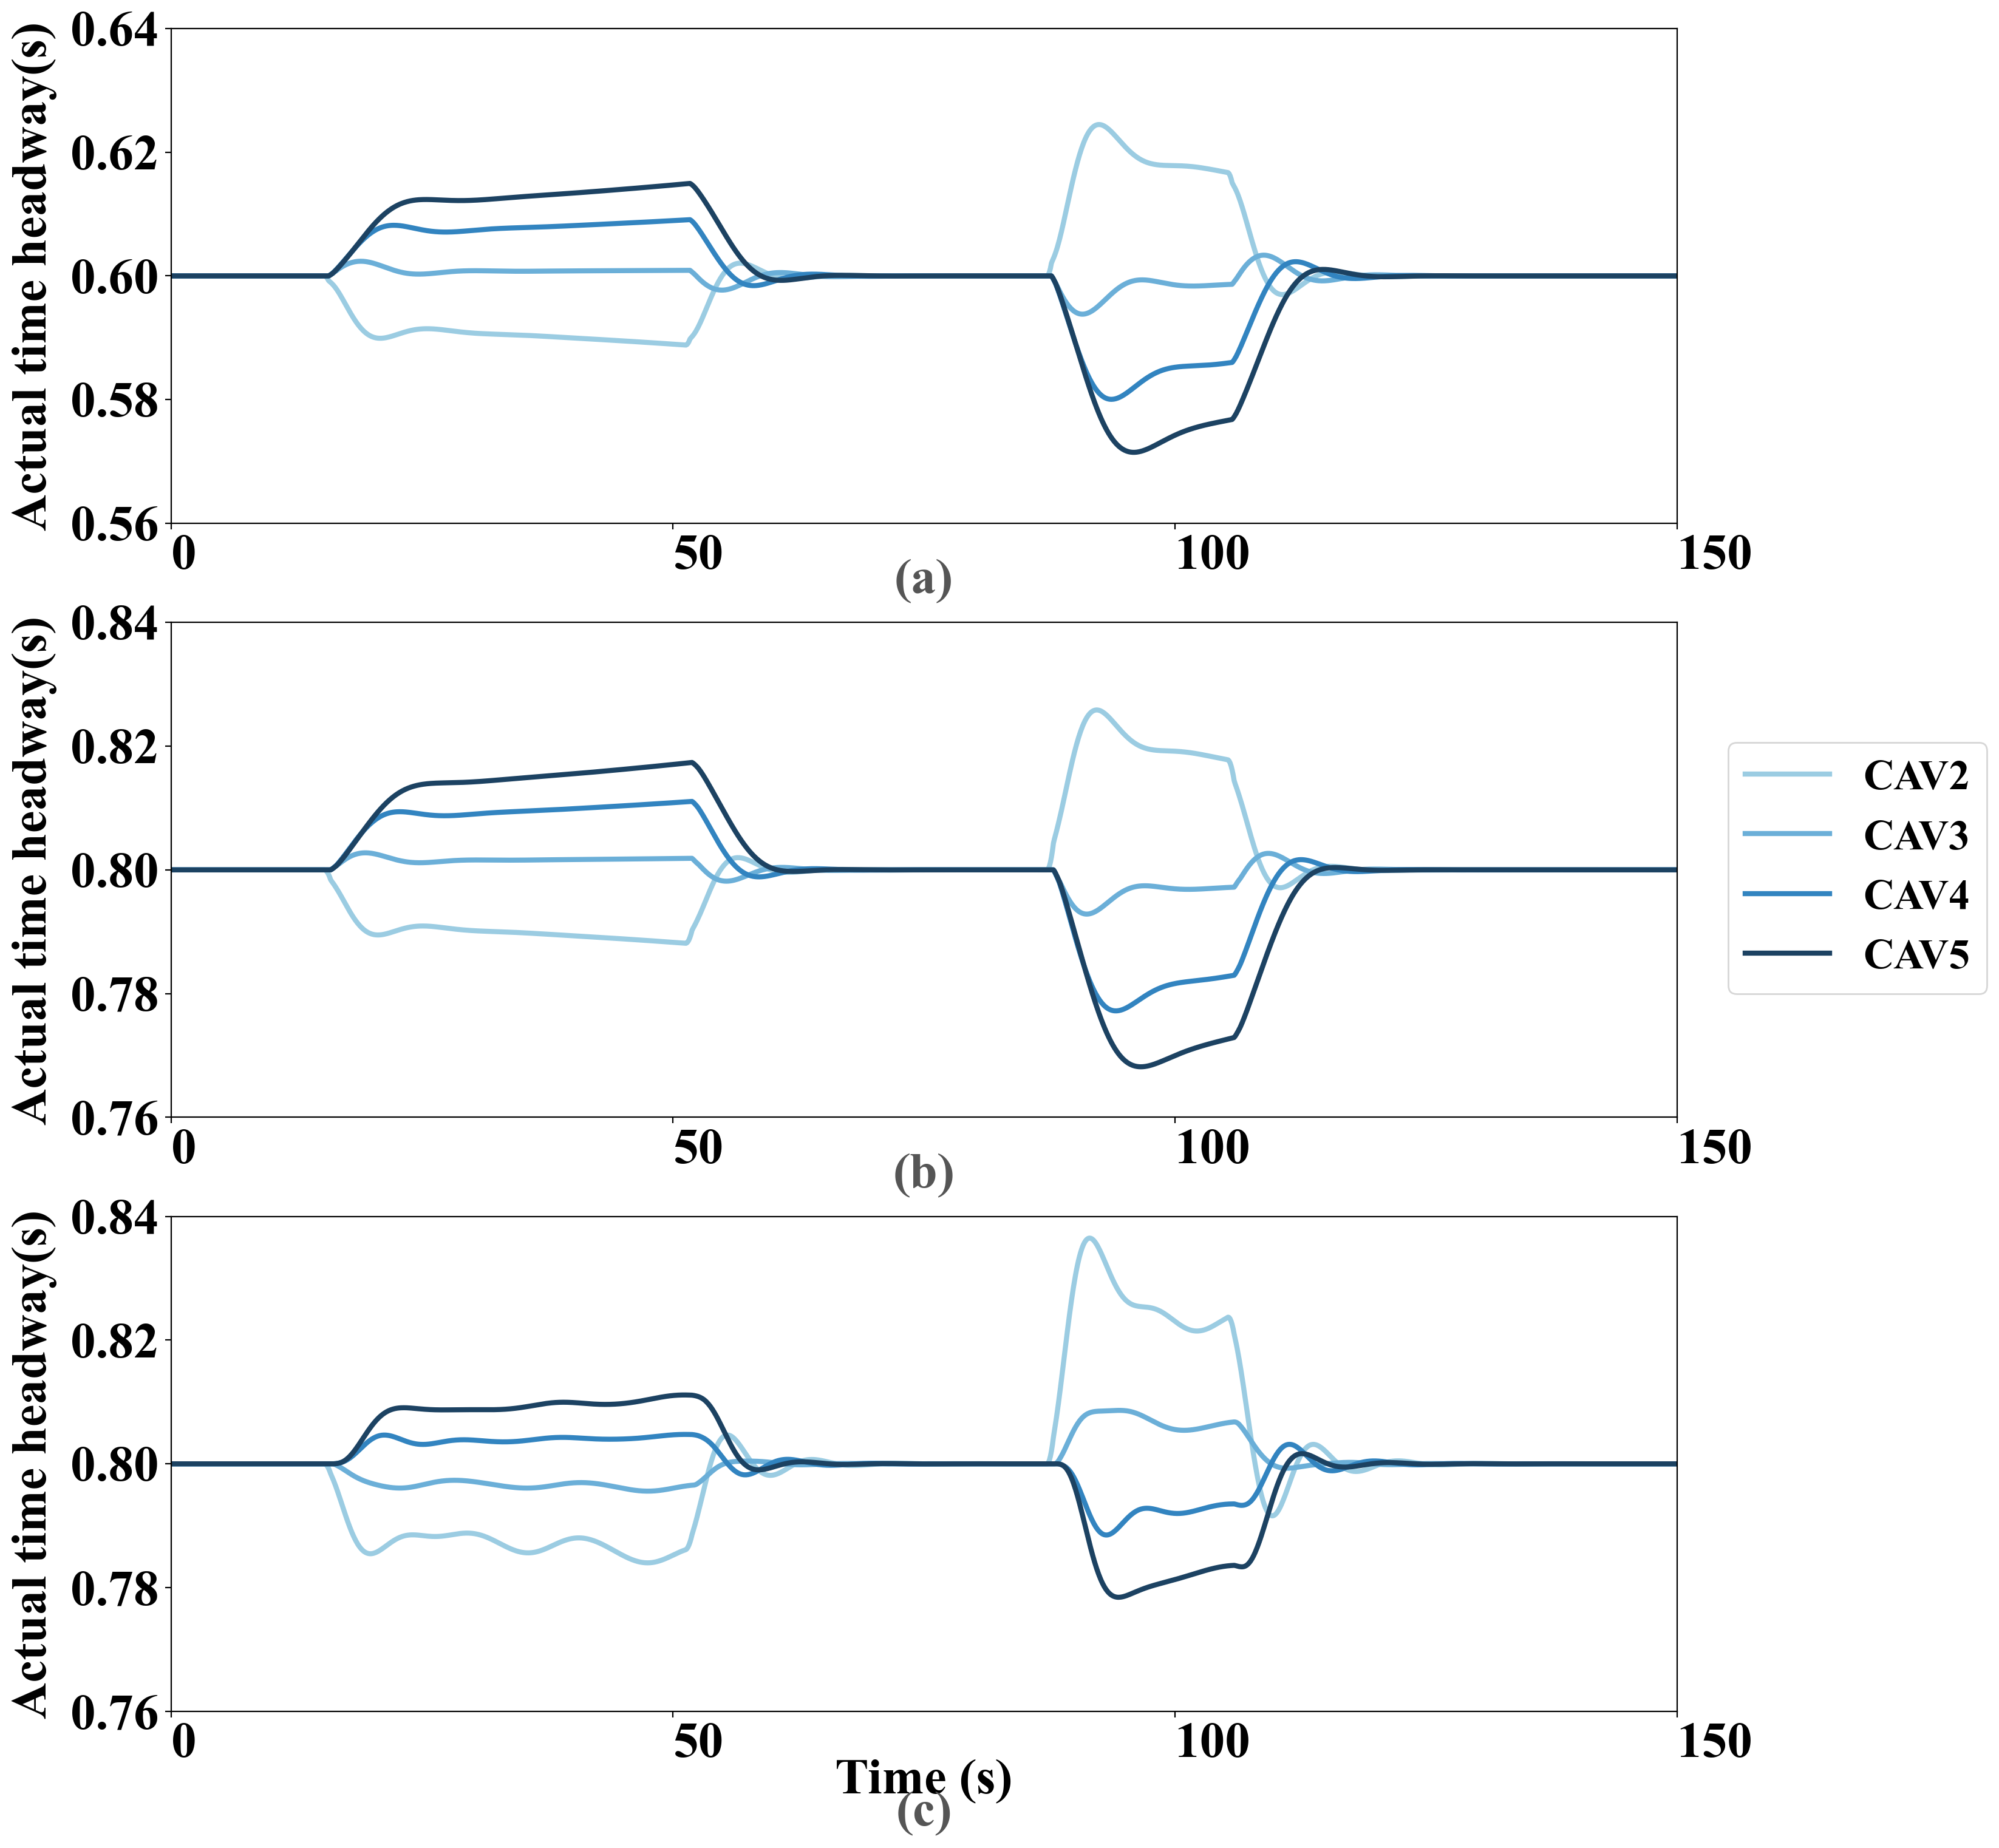
\includegraphics[width=8.5cm]{figs/fig6.png}
  \caption{~The variation of actual time headway with time for the three cases under the Trapezoidal signal in Fig.~\ref{fig2}(a,b): (a) Case \uppercase\expandafter{\romannumeral1}; (b) Case \uppercase\expandafter{\romannumeral2}; (c) Case \uppercase\expandafter{\romannumeral3}.}
  \label{fig6}
\end{figure}

The above analyses seem to conclude that ignoring the internal communication delay does not significantly affect the tracking performance. However, this conclusion can be falsified by comparing the actual time headway of different cases shown in Fig.~\ref{fig6}. Although the desired time headway of each CAV is set to $0.6s$ in each case, the actual time headway is not kept at $0.6s$ but $0.8s$ in Case \uppercase\expandafter{\romannumeral2} and Case \uppercase\expandafter{\romannumeral3} due to the presence of the internal communication delay. In other words, internal communication delay does not directly worsen the tracking performance. However, it prolongs the actual time headway leading to a deterioration of the capacity, which is believed to achieve better tracking performance if the actual time headway is longer. In addition, comparing the actual time headway of different CAVs under perturbation, it is observed that the actual time headway of CAV2 is lower than the desired time headway in the deceleration phase and higher in the acceleration phase, unlike the other CAVs. This phenomenon is due to the delays in the deceleration phase, which causes the subsequent CAVs to decelerate more slowly compared to the leader, resulting in a velocity greater than the leader. Therefore, the spacing between the two becomes smaller, leading to the actual time headway of CAV2 being lower than the desired time headway. For the other CAVs, the leader-based communication makes the difference between the CAVs insignificant, although also due to the presence of delay compared to the Leader's slower deceleration. Similarly, the variation of the actual time headway during the acceleration phase can be explained by the above reasons.
% \clearpage
\subsubsection{Safety analyses under the hard braking maneuver}
\label{Section 5.2.2}

To investigate the effect of internal communication delay and time-varying structured uncertainties on safety, another quantitative analysis is conducted for the hard braking maneuver scenario, considered one of the most traffic accident-prone scenarios \citep{Taheri1990,Saito2016,zhang2015all}. In the hard braking scenario, the leader decelerates from $20m/s$ to $0m/s$ within the $20s$. Moreover, here we select the Deceleration Rate to Avoid the Crash (DRAC) as the safety indicator, which presents the deceleration rate needed by a vehicle to avoid a collision with another vehicle. The DRAC can be defined for each vehicle $i$ at the time $t$ as follows:
\begin{equation*}
  DRAC{_i}(t) = \frac{{{{\left( {{v_i}(t) - {v_{i - 1}}(t)} \right)}^2}}}{{2\left( {{p_{i - 1}}(t) - {p_i}(t) - L} \right)}}
\end{equation*}

\begin{figure}
  \centering
  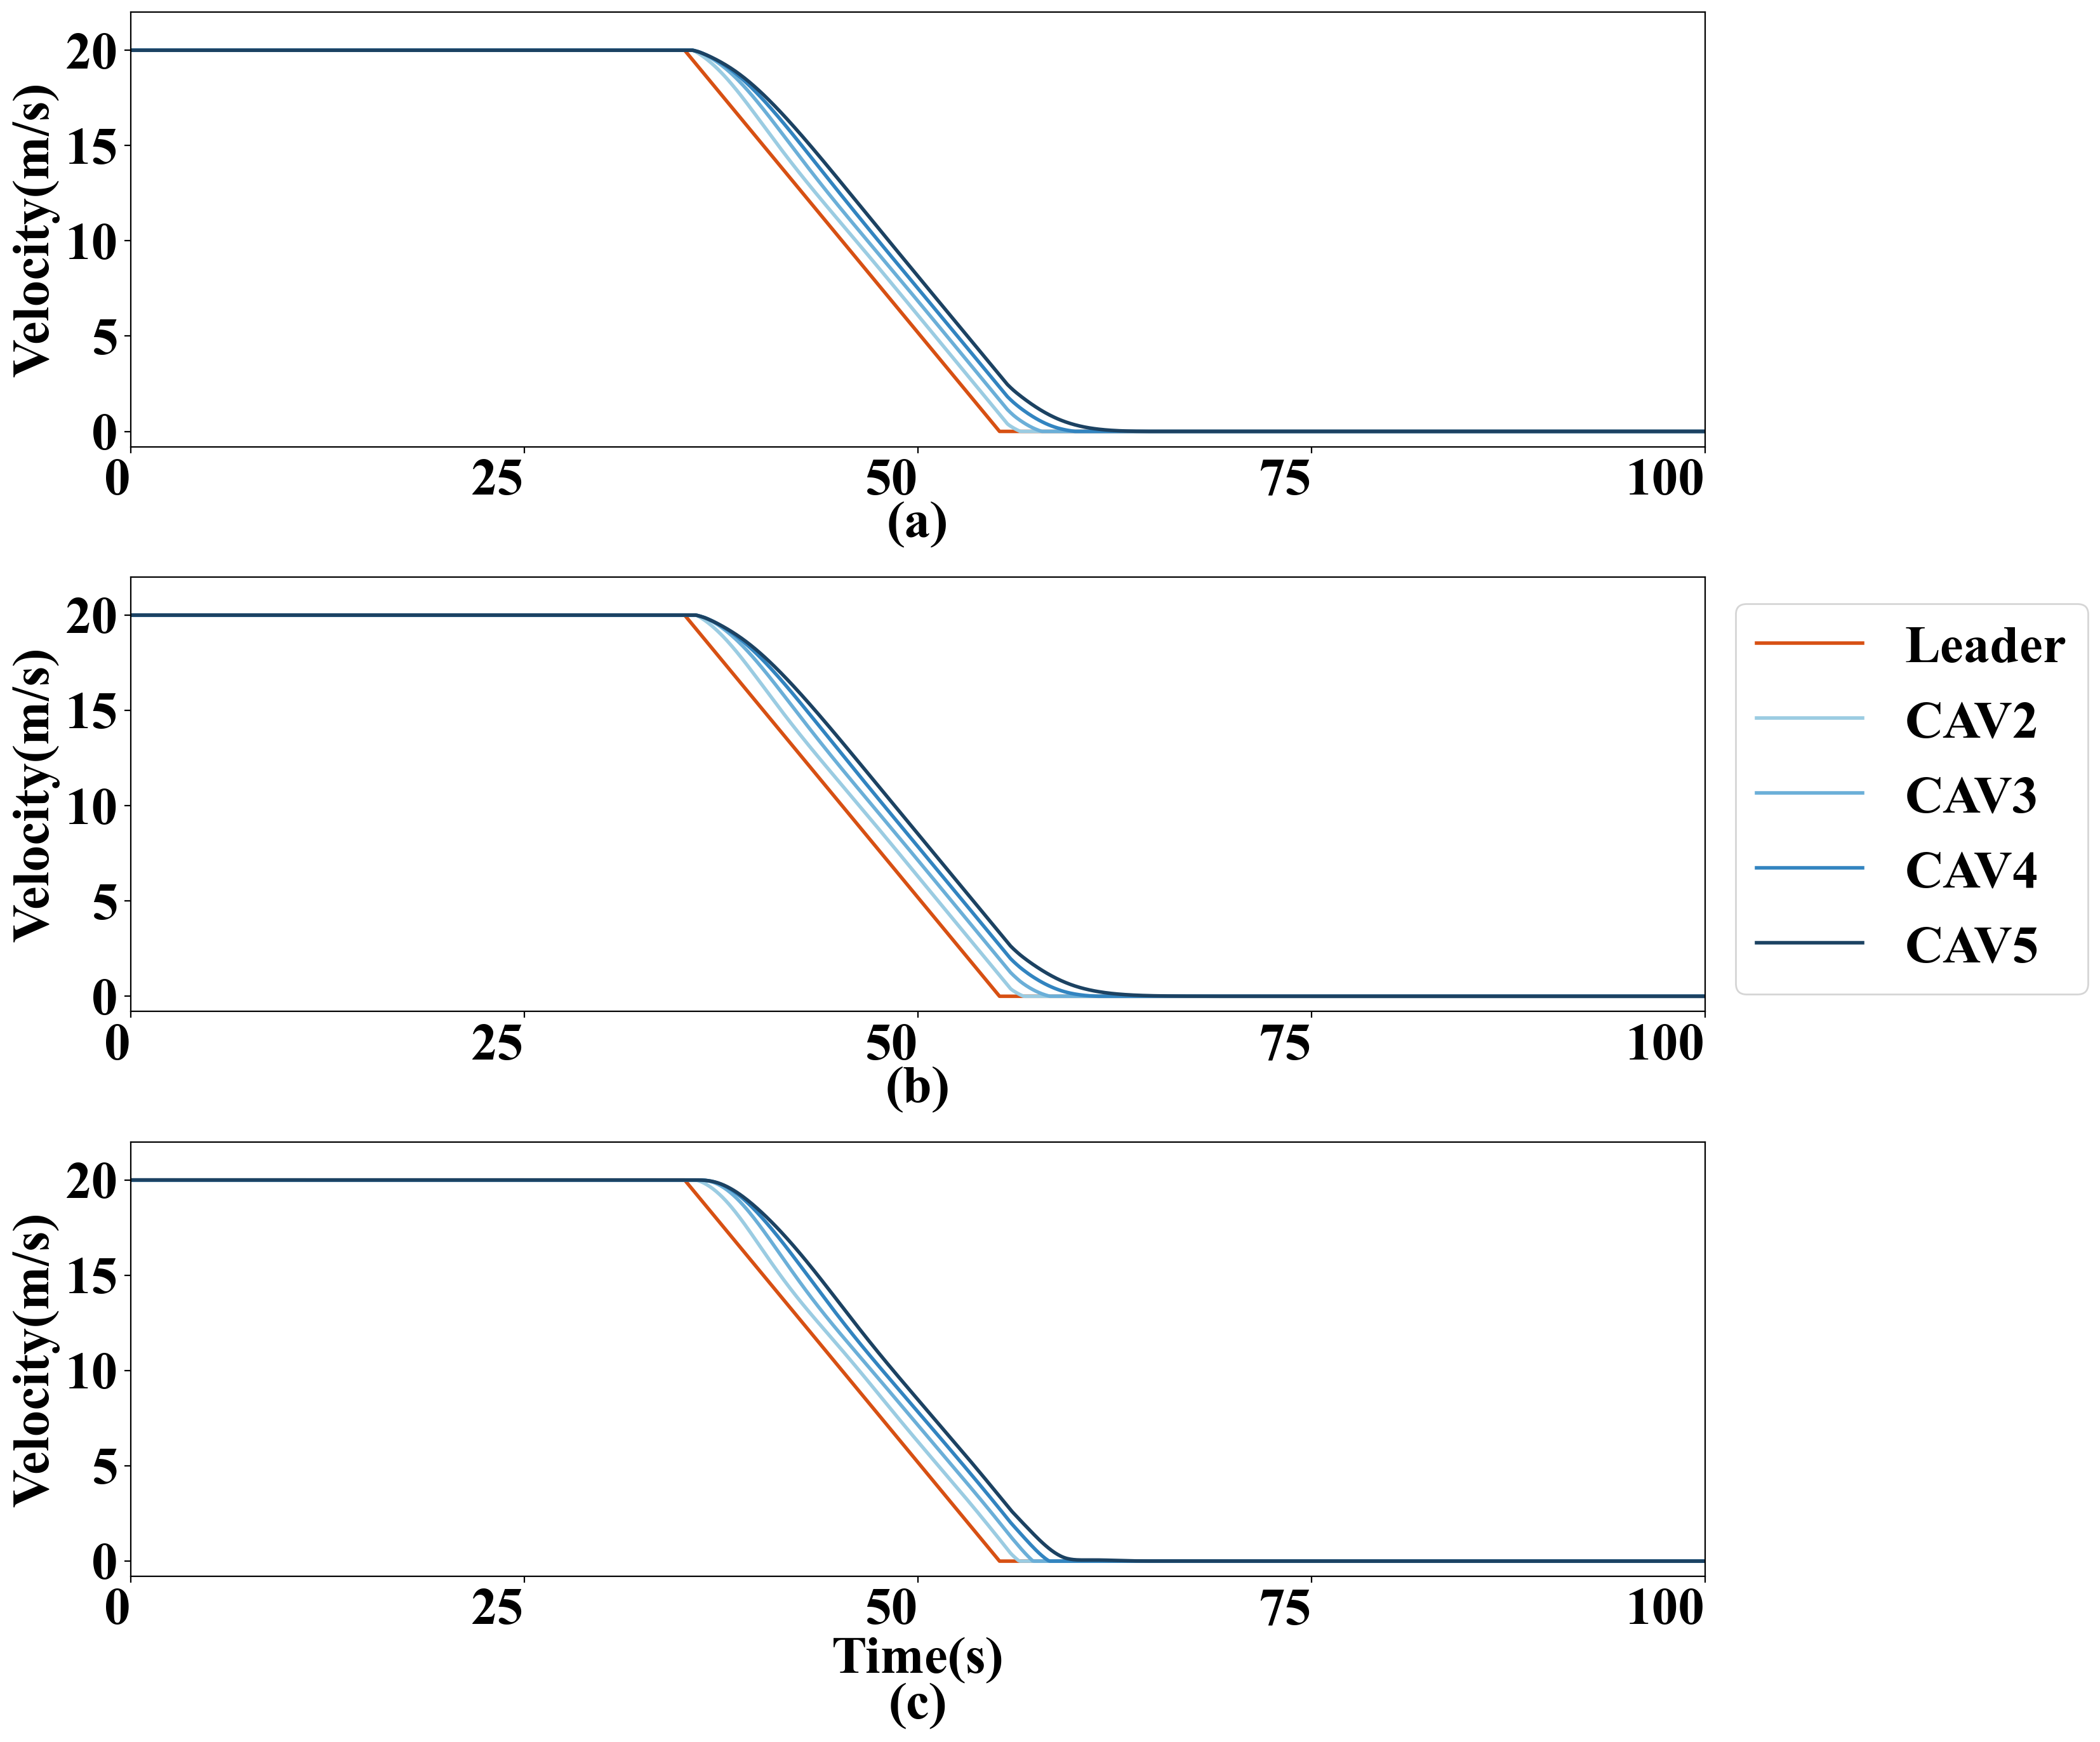
\includegraphics[width=8.5cm]{figs/fig7.png}
  \caption{~Tracking performances for a hard braking maneuver: (a) Case \uppercase\expandafter{\romannumeral1}; (b) Case \uppercase\expandafter{\romannumeral2}; (c) Case \uppercase\expandafter{\romannumeral3}.}
  \label{fig7}
\end{figure}

Fig.~\ref{fig7} illustrates how the CAV platoon tracks the leader motion under the hard braking maneuver for the three cases. Likewise, the CAV platoon, in any case, is capable of tracking the leader motion smoothly and avoiding collisions. Further, the DRAC of each CAV in the platoon is depicted as box plots in Fig.~\ref{fig8}, where the CAV2, CAV3, CAV4, and CAV5 refer to the second, third, fourth, and fifth CAV in the CAV platoon, respectively. One conclusion can be drawn that the introduction of uncertainties significantly increases the DRAC making collision-prone scenarios more probable, similar to the rough results obtained in the tracking performance analyses. Specifically, the DRAC of CAV2 in Case \uppercase\expandafter{\romannumeral1} and Case \uppercase\expandafter{\romannumeral2} is only $84.48\%$ and $82.76\%$ of that in Case \uppercase\expandafter{\romannumeral3}, respectively. Meanwhile, considering the internal communication delay has an unremarkable effect on the DRAC. Furthermore, another conclusion can be drawn by comparing different CAVs in the same case. That is, the indexes in the platoon influence the safety conditions, even though the control parameters are the same.

\begin{figure}
  \centering
  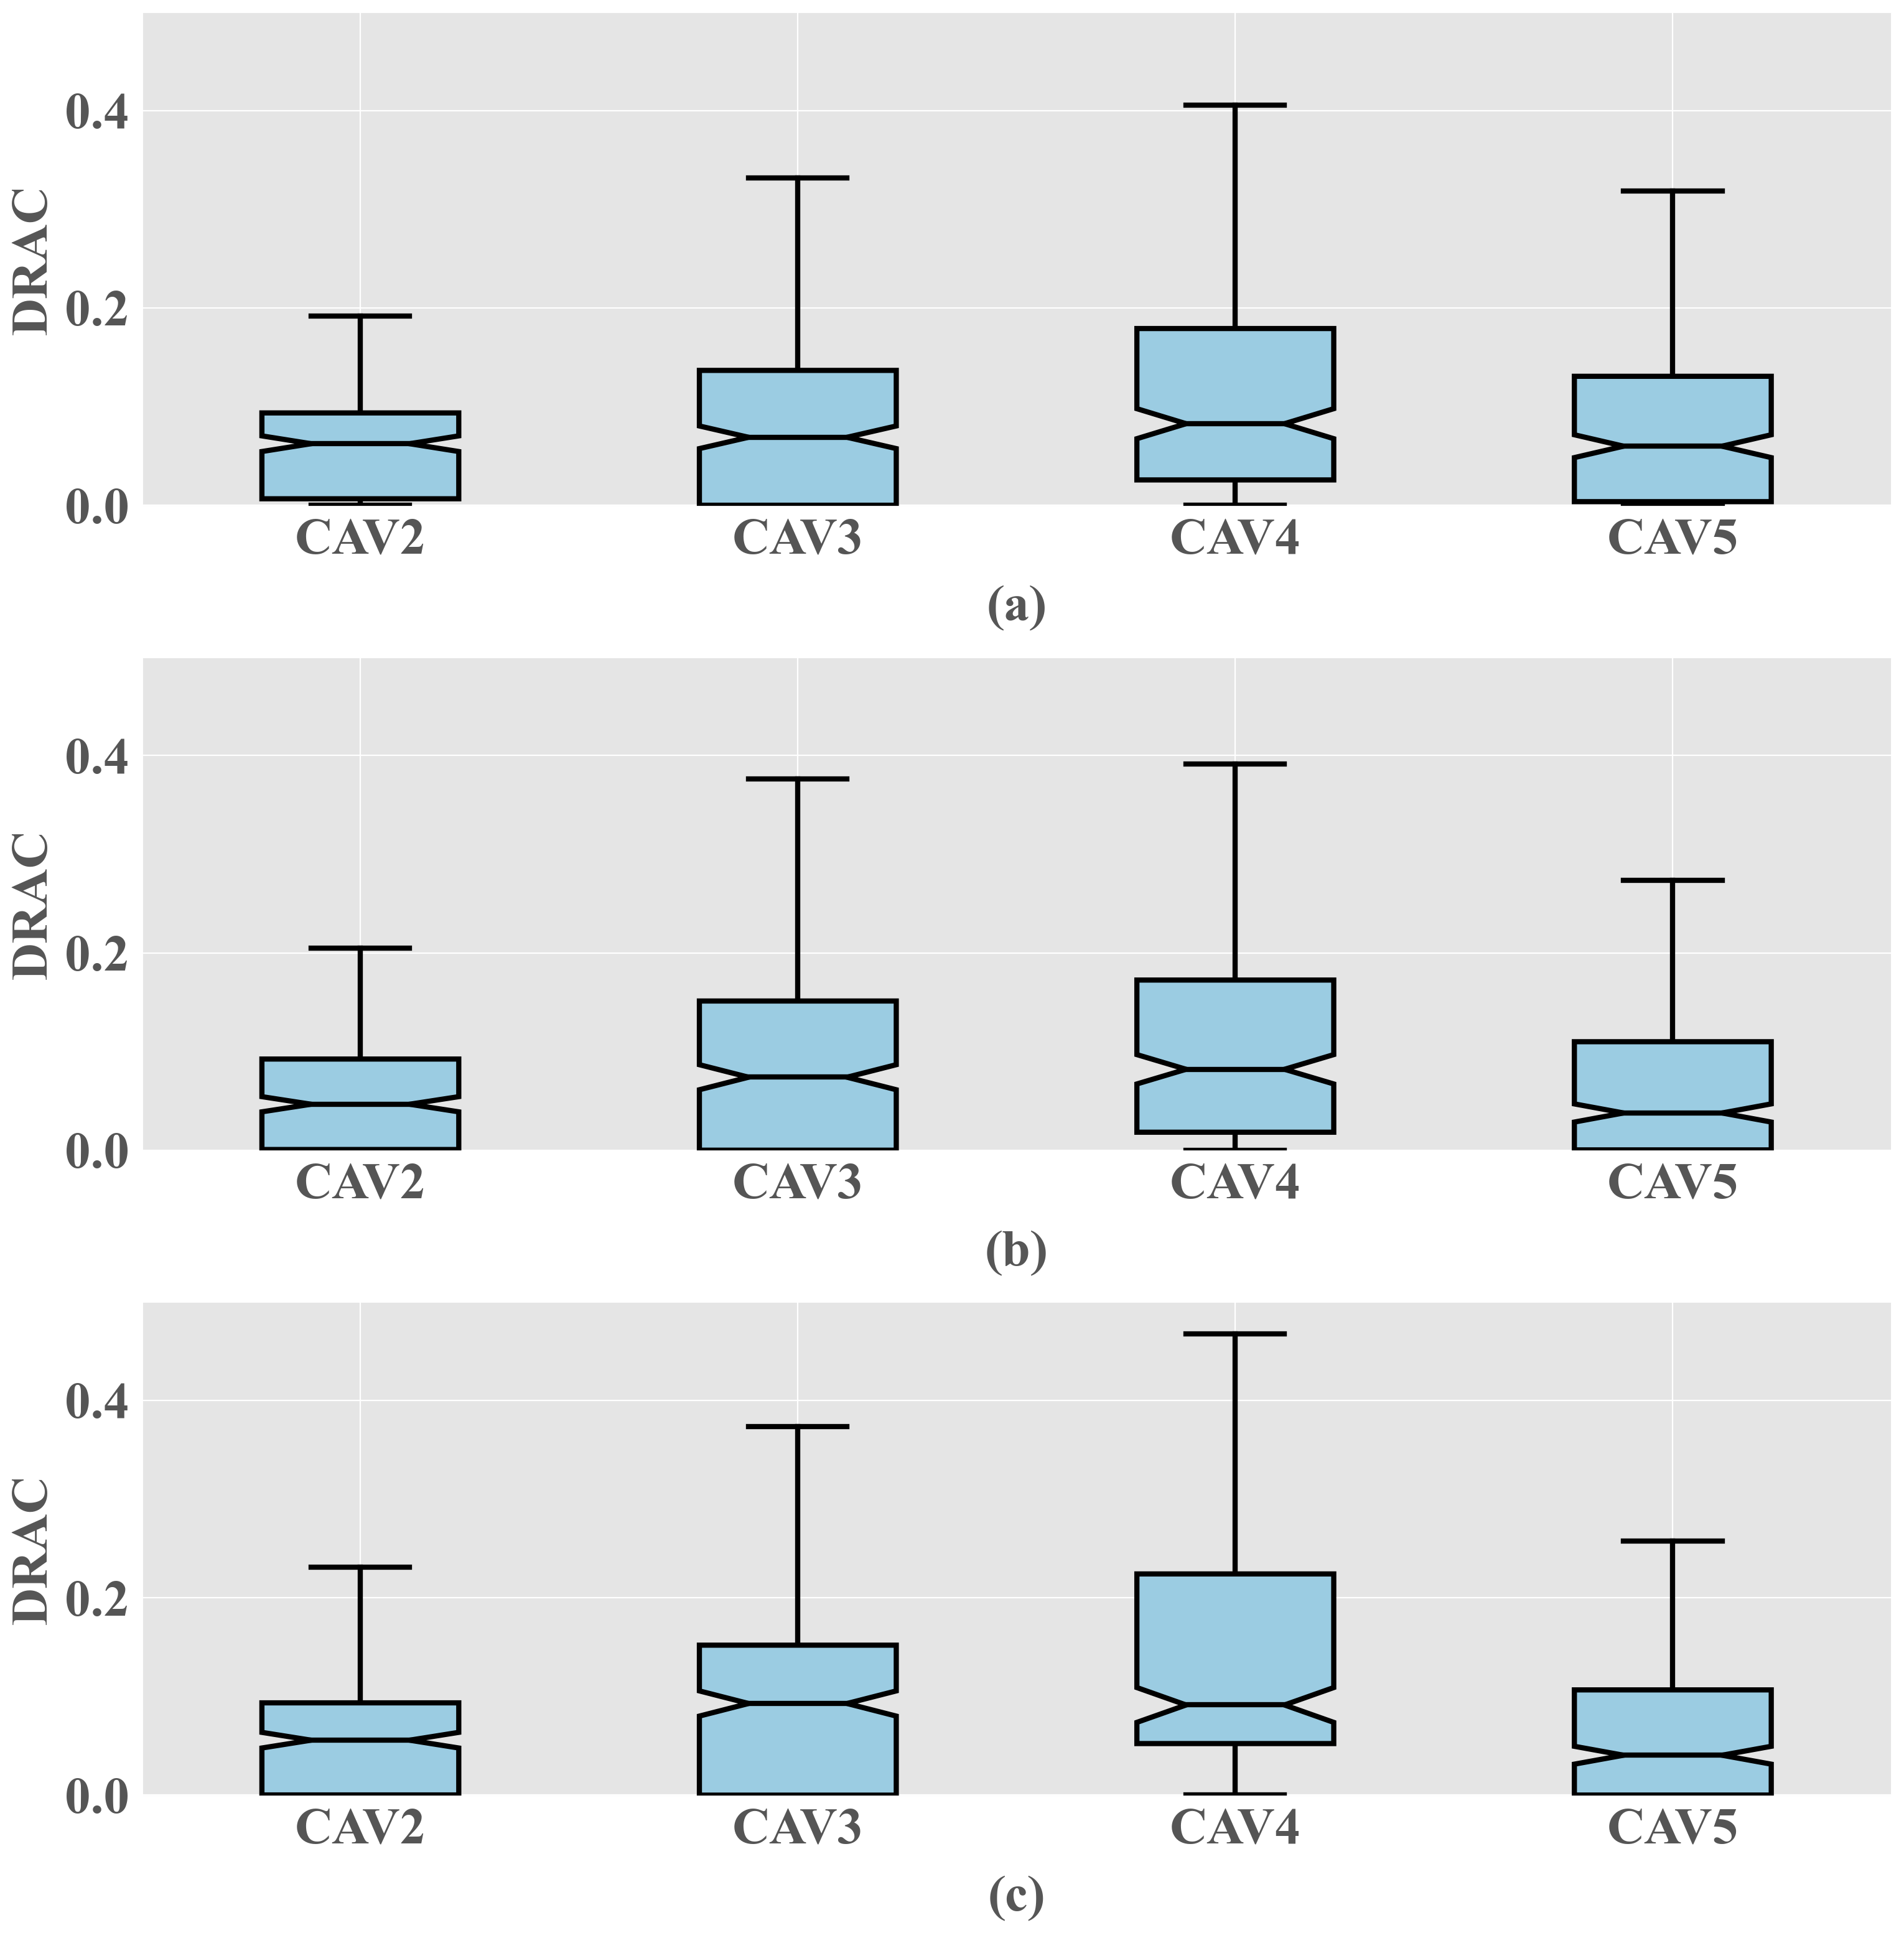
\includegraphics[width=8.5cm]{figs/fig8.png}
  \caption{~The DRAC boxplots of each CAV for the three cases: (a) Case \uppercase\expandafter{\romannumeral1}; (b) Case \uppercase\expandafter{\romannumeral2}; (c) Case \uppercase\expandafter{\romannumeral3}.}
  \label{fig8}
\end{figure}

% \clearpage
\subsection{Numerical analyses of the CAV platoon under different control parameters}
\label{Section 5.3}

In this subsection, the parameters in Table~\ref{table1} are still adopted for both network and traffic simulation. Moreover, in order to investigate the effect of different feedback control gains on tracking performance, the following four feedback control gains are selected:
\begin{enumerate}
  \item \textit{Parameter \uppercase\expandafter{\romannumeral1}:} $ {k_i} = {[0.3,0.3,0.3]^T} $;
  \item \textit{Parameter \uppercase\expandafter{\romannumeral2}:} $ {k_i} = {[0.5,0.3,0.3]^T} $;
  \item \textit{Parameter \uppercase\expandafter{\romannumeral3}:} $ {k_i} = {[0.3,0.5,0.3]^T} $;
  \item \textit{Parameter \uppercase\expandafter{\romannumeral4}:} $ {k_i} = {[0.3,0.3,0.5]^T} $.
\end{enumerate}
Moreover, corresponding matrixes $P,Q_i,W_j,A_{ij},B_{ij},C_{ij}$ with $i=1,2,3,i<j\le3 $satisfying Theorem~\ref{theorem7} can be found in Appendix E.

As in Section~\ref{Section 5.2.1}, the Trapezoidal signal defined in Section~\ref{Section 5.1} is employed to investigate the tracking performances of different control parameters. The tracking performances of the CAV platoon are presented in Fig.~\ref{fig9}.

\begin{figure}
  \centering
  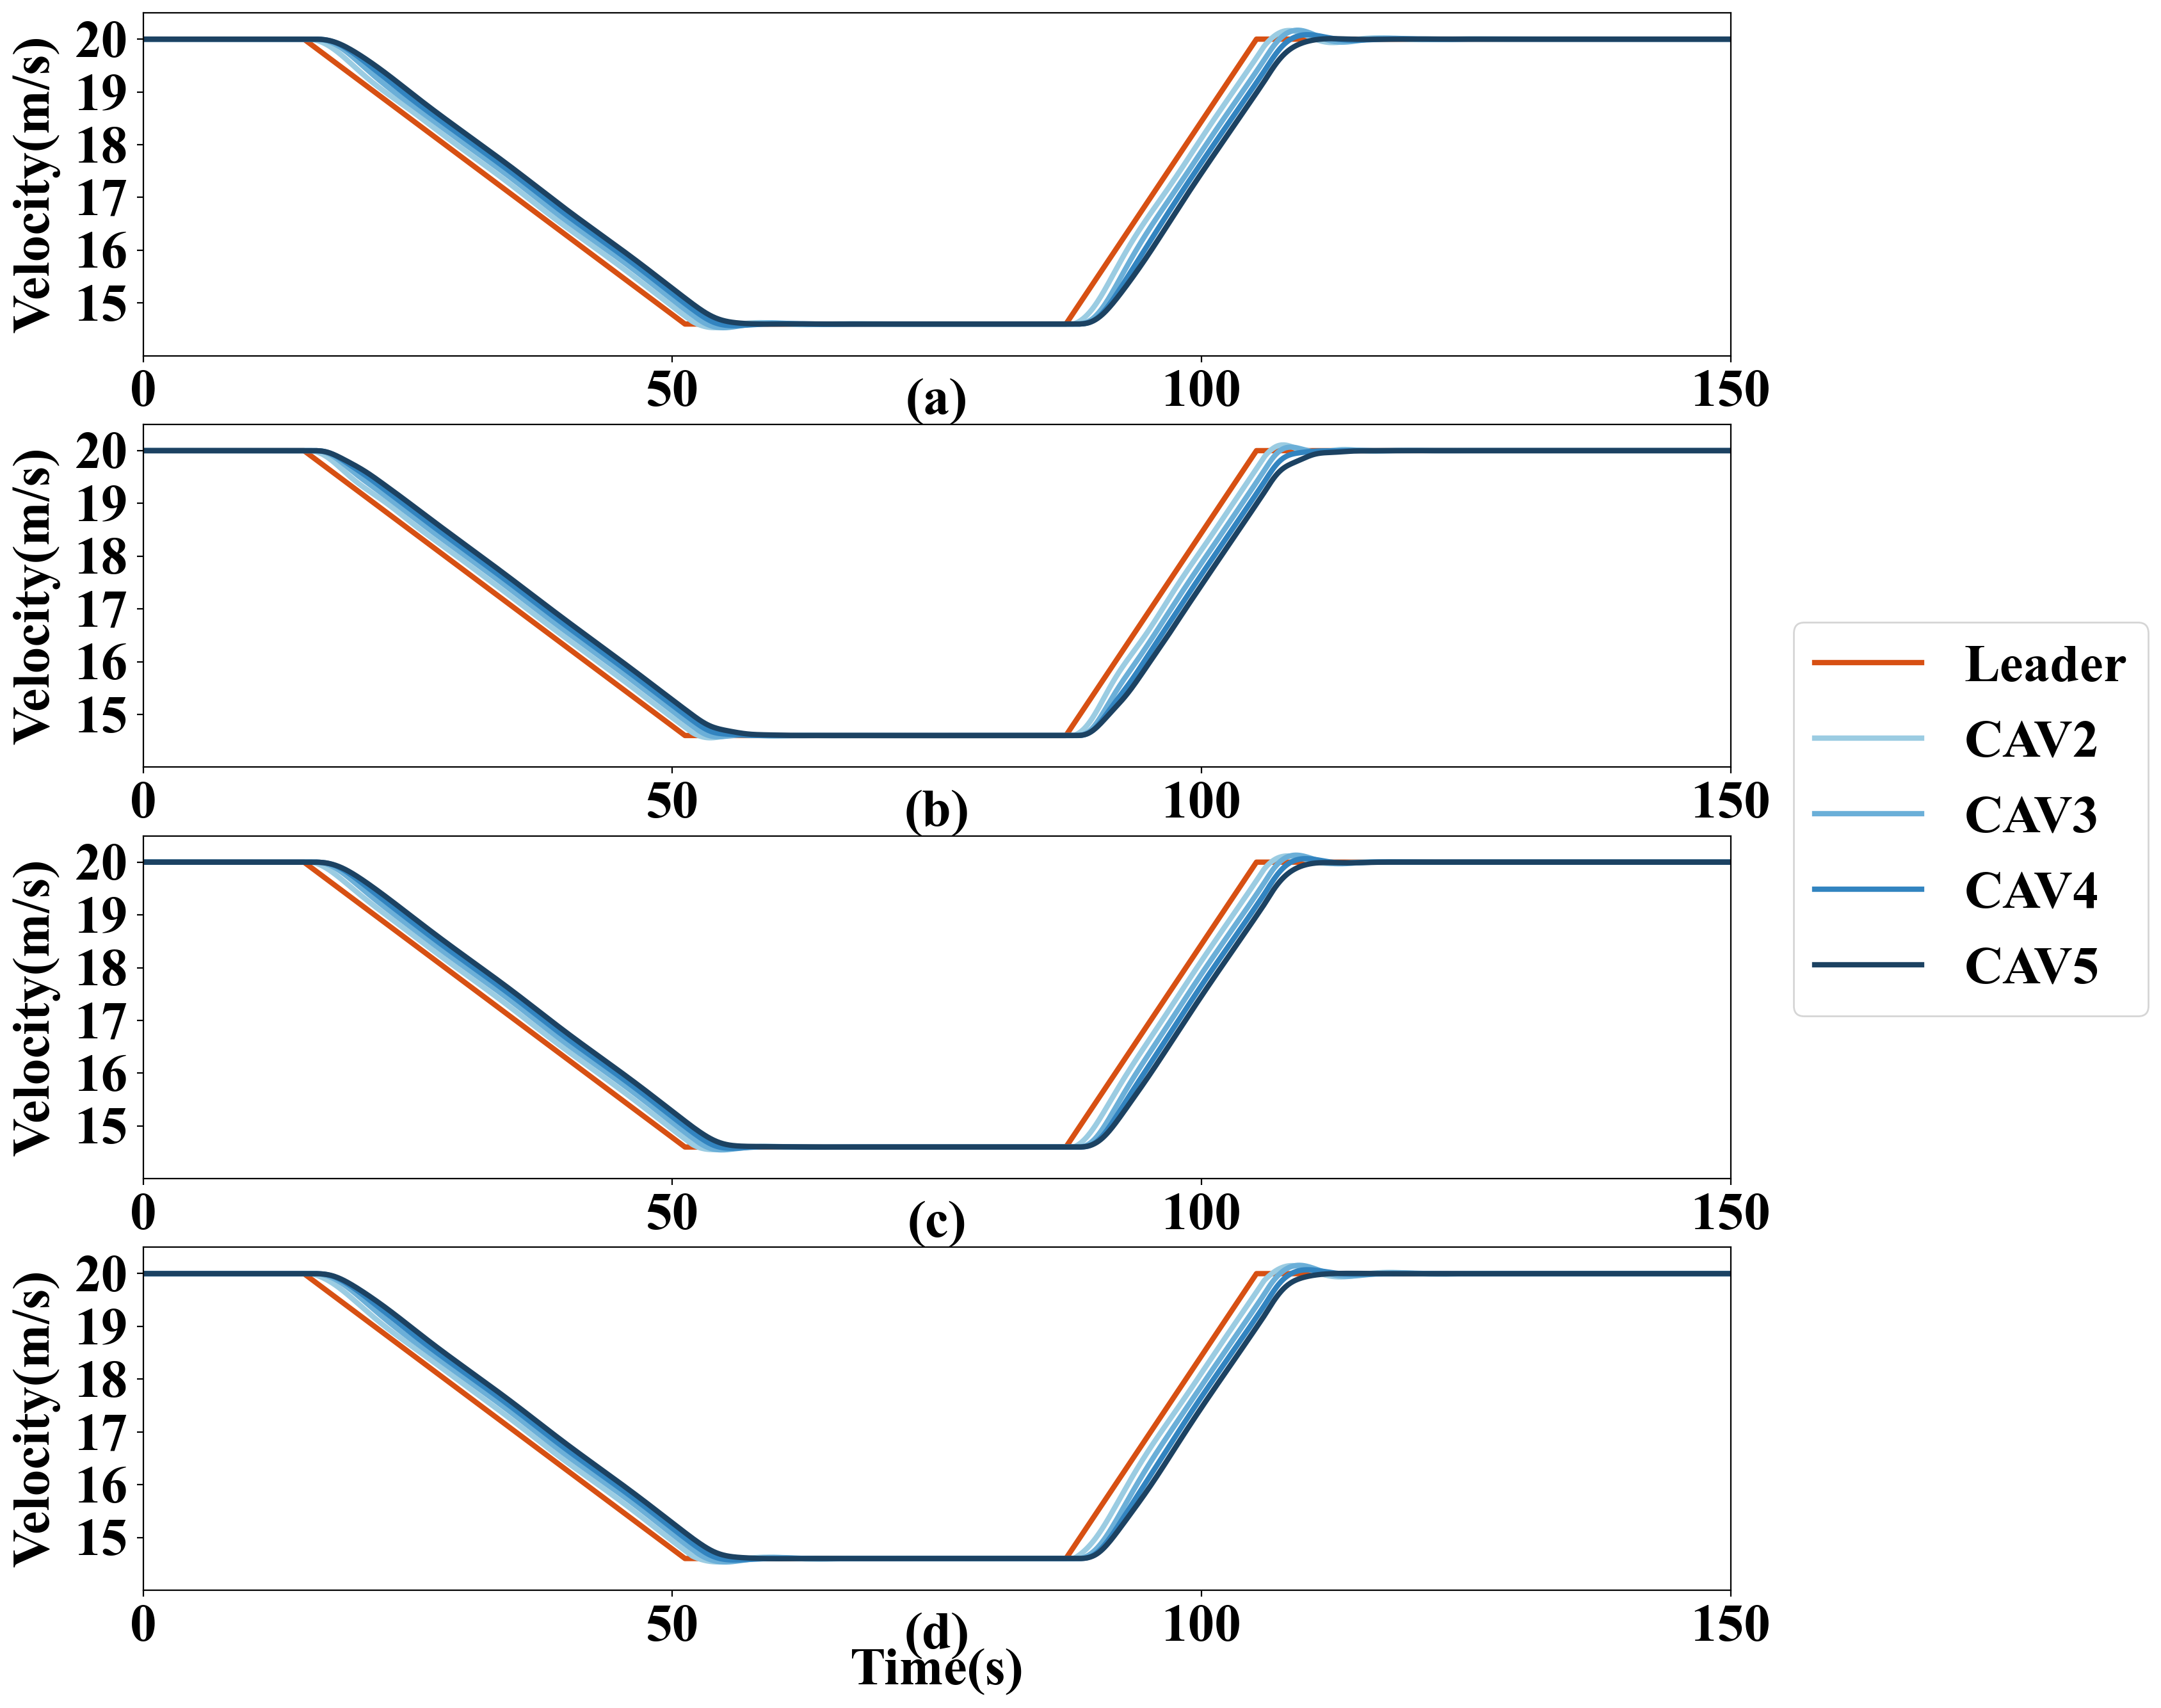
\includegraphics[width=8.5cm]{figs/fig9.png}
  \caption{~Tracking performances of the CAV platoon for the Trapezoidal signal in Fig. 3(a,b) under different parameters: (a) presents tracking results under \textit{Parameter \uppercase\expandafter{\romannumeral1}}; (b) presents tracking results under \textit{Parameter \uppercase\expandafter{\romannumeral2}}; (c) denotes the case under \textit{Parameter \uppercase\expandafter{\romannumeral3}}; (d) denotes the case under \textit{Parameter \uppercase\expandafter{\romannumeral4}}.}
  \label{fig9}
\end{figure}

Good tracking performances have also been verified for different control parameters. A similar phenomenon can be observed that the transient response from tracking Leader motion decreases gradually, thanks to stability.

\begin{figure}
  \centering
  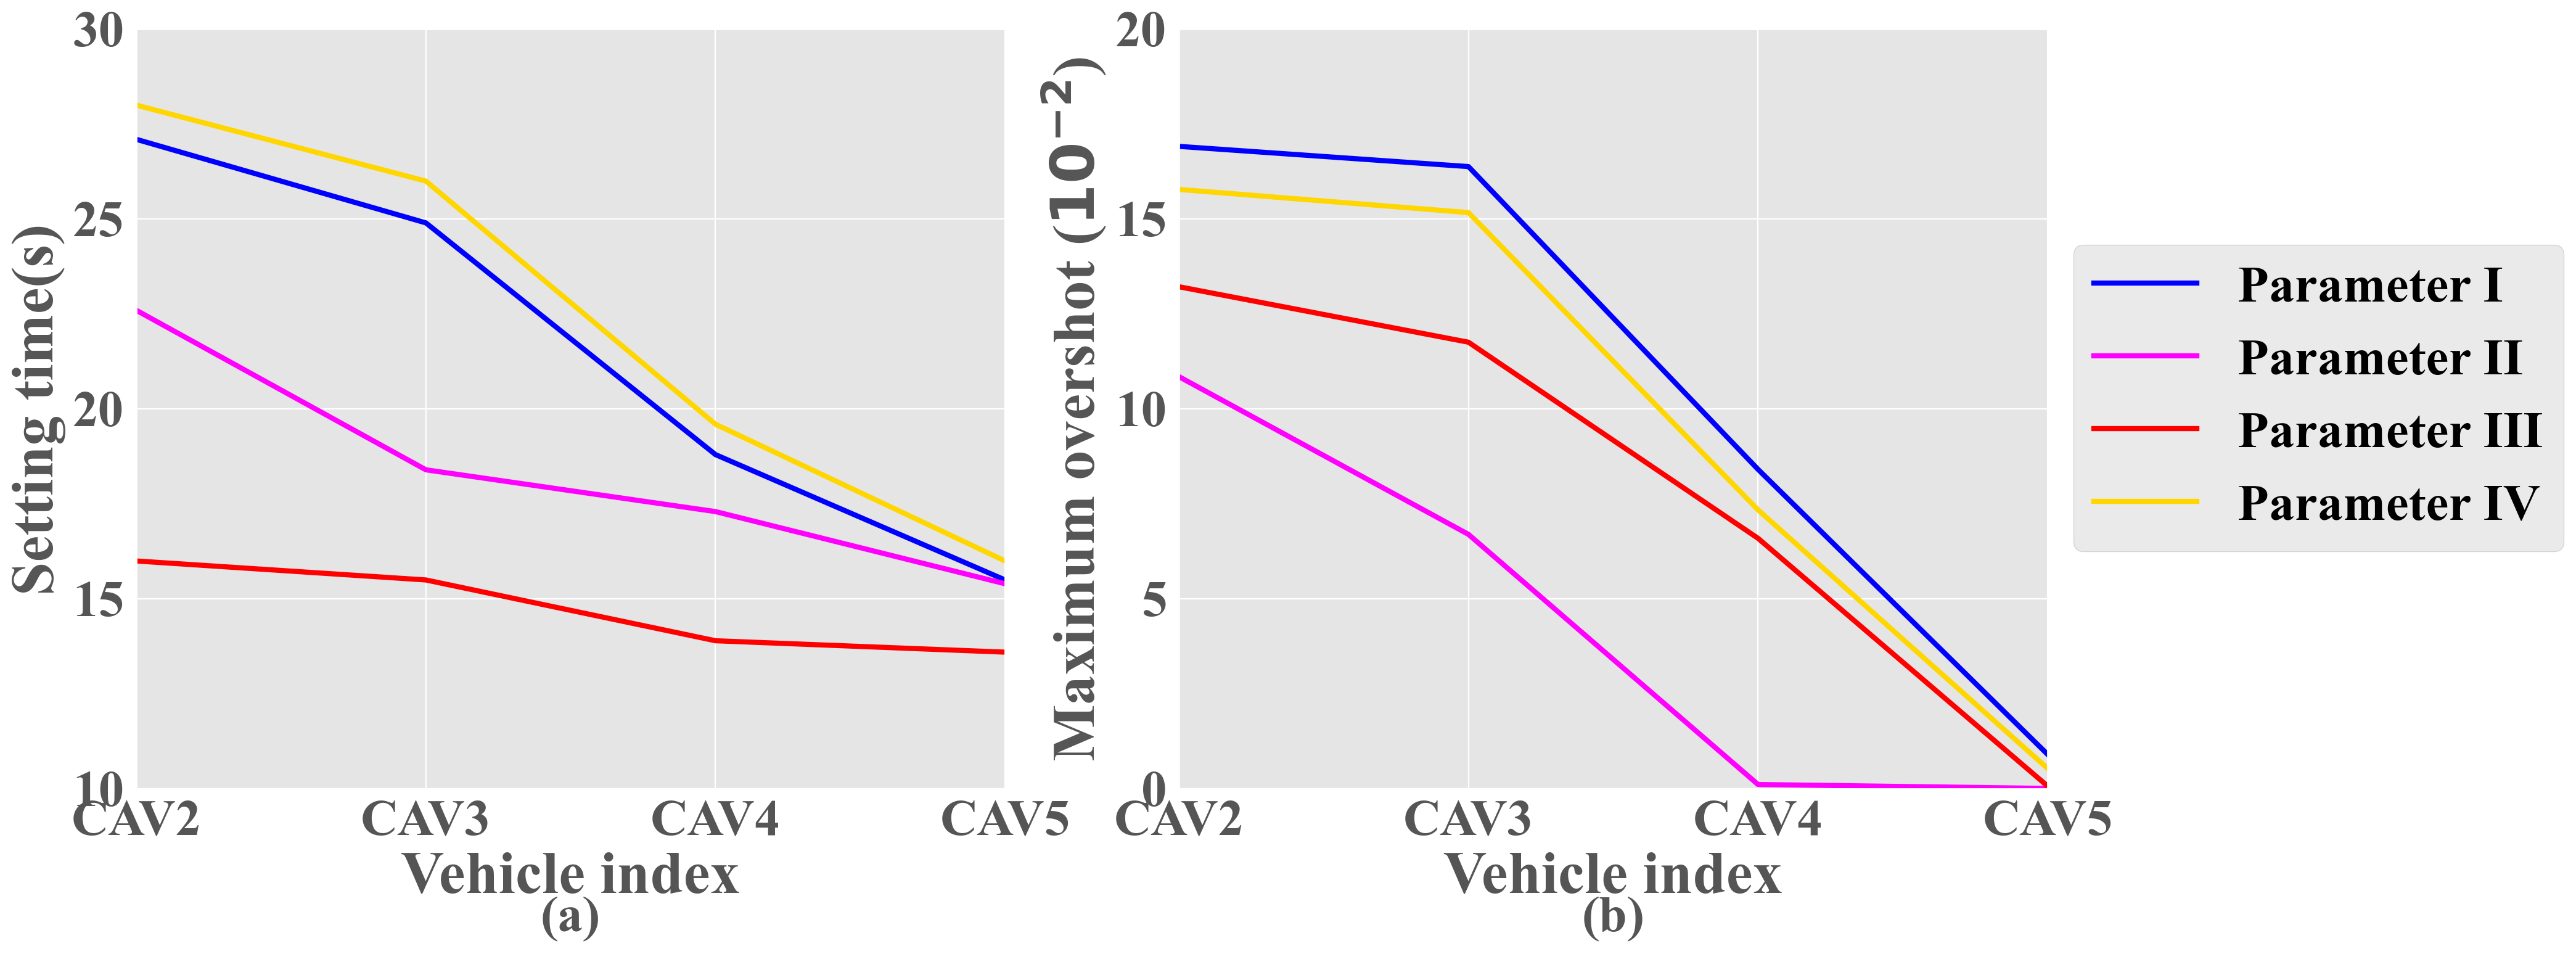
\includegraphics[width=8.5cm]{figs/fig10.png}
  \caption{~Indicators for evaluating the transient response of each CAV among the CAV platoon under the four control parameters: (a) the case of setting time; (b) the case of the maximum overshoot.}
  \label{fig10}
\end{figure}

Similarly, ST and MO are analyzed to investigate the specific effects of different control parameters on the transient response, and the results are demonstrated in Fig.~\ref{fig10}. One conclusion can be drawn that different control gains affect the transient response. Comparing the case of different control gains, the cases of Parameter \uppercase\expandafter{\romannumeral2} and Parameter \uppercase\expandafter{\romannumeral3} have a smaller ST and MO than the case of Parameter \uppercase\expandafter{\romannumeral1}, which indicates that improving the gain of spacing and velocity errors is indeed effective in reducing the velocity fluctuations and time from the perturbation to the equilibrium state, thus improving driving comfort and safety. However, the results of the Parameter \uppercase\expandafter{\romannumeral4} show that increasing the gain of acceleration error is not a good idea to improve the transient response since it raises the ST despite lowering the MO. Furthermore, for all cases of control gain, the ST and MO decrease as the vehicle index increases, which leads to a similar conclusion as in Section~\ref{Section 5.2.1}. It is worth mentioning that for the case of Parameter \uppercase\expandafter{\romannumeral2}, the MO is 0 means that the transient response under this case is not overshoot, which is an excellent benefit on safety and comfort.

% \clearpage
% \begin{equation}
%   \label{eq}
% \end{equation}
% \citep{Vukadinovic2018a,Wang2018e}
% \citep{ogata1995discrete}

% \citep{Taheri1990,Saito2016,zhang2015all}
% \begin{table}
%   \centering
%   \setlength{\abovecaptionskip}{0pt}
%   \setlength{\belowcaptionskip}{10pt}%设置标题与表格的距离
%   \begin{threeparttable}[b]

%     \caption{~Network and traffic simulation parameters.}
%     \label{table1}
%     {\begin{tabular}{lc} \toprule
%         Parameters                                         & Value               \\ \midrule
%         Platoon size $n$                                   & 5 vehicles          \\
%         \bottomrule
%       \end{tabular}}
%     \begin{tablenotes}
%       \item[1] \citep{Wang2018a,Zhou2020}
%     \end{tablenotes}
%   \end{threeparttable}
% \end{table}


\section{Conclusion and future work}
\label{Section 6}

This paper proposes a general modeling approach for the CAV platoon, considering multiple time delays. This general modeling approach consists of applying graph theory to describe the communication relationships within a CAV platoon generally defined by IFT and modeling the linear time-invariant state time-varying delay system corresponding to the CAV platoon that employs a CTH control strategy. Furthermore, based on the properties of the linear time-invariant system with multiple state delays, a novel stability criterion of the general CAV platoon is derived based on Lyapunov-Krasovskii Stability Theorem and free-weighting matrix. In addition, considering the existence of system uncertainties, a stability criterion that takes time-varying structured uncertainties into account is also derived. Furthermore, extensive numerical analyses are conducted to comprehensively evaluate the tracking performances and safety conditions of the CAV platoon, considering the multiple delays and measuring uncertainties. At last, comparing the tracking performances between the CAV platoons adopting different control parameters sheds some light on the selection of control parameters.
The following conclusions can be drawn through numerical analysis:
\begin{enumerate}

  \item With the help of the Lyapunov-Krasovskii stability theorem and free-weighting matrix, a stability criterion considering the multiple delays for the CAV platoon can be obtained.
  \item All CAVs under each case can smoothly track errors and return to equilibrium if the stability criterion is satisfied.
  \item  The introduction of time-varying structured uncertainties and the internal communication delay worsens the tracking performance. The difference is that time-varying structured uncertainties lead to more significant overshoot and recovering time, and the internal communication delay makes CAV unable to perform the desired time headway.
  \item The more realistic scenarios with the introduction of time-varying structured uncertainties have worse safety conditions than the ideal case. Specifically, the mean value of DRAC without uncertainties is only $82.76\%$ of the case with uncertainties, making collision-prone scenarios more probable.
  \item Different control parameters have a significant impact on tracking performances. Furthermore, increasing the gain of spacing and velocity errors can benefit tracking performance, while increasing the gain of acceleration errors does not.

\end{enumerate}

However, it should be admitted that the results obtained from the simulation are only a simplification of reality, so field experiments are necessary to further investigate the tracking performances in the future. In addition, the communication delay is assumed to be a constant upper bound for simplicity in this paper. Nevertheless, the communication delay is time-varying and varies with the surrounding environment, thus introducing conservatism. Therefore, corresponding stability criteria for dealing with time-varying delays must be developed. In addition, theoretical research and field experiments should be conducted to investigate control parameter schemes that yield the best tracking performance. Furthermore, future research should also focus on designing new control strategies to achieve smoother and safer tracking performance.

\appendix


\section*{Appendix A.~Feedback control for linearization}
\label{AppendixA}
In this appendix, we provide the linearization of the longitudinal vehicle dynamic in Equation~(\ref{eq1}). The functions of the lumped uncertain resistance forces, including $f_i^g(t)$, $f_i^w(t)$, and $f_i^r(t)$ are expressed as follows:

\begin{equation}
  \left\{\begin{array}{l}
    f_{i}^{g}(t)=m_{i} g \sin \left(\theta_{i}(t)\right),                         \\
    f_{i}^{w}(t)=\frac{1}{2} \rho C_{D} A_{F}\left(v_{i}(t)+v_{w}(t)\right)^{2} , \\
    f_{i}^{r}(t)=\mu_{R} m_{i} g \cos \left(\theta_{i}(t)\right),
  \end{array}\right.
  \label{eqA1}
\end{equation}
where $g=9.81m/s^2$ denotes the acceleration of gravity; $\theta_i(t)$ is the inclination angle of the road; $\rho$ denotes the air density; $C_D$ is the aerodynamic drag coefficient; $A_F$ represents the maximal cross-sectional/frontal area of the vehicle; $v_w(t)$ denotes the uncertain headwind speed; $\mu_R$ is the coefficient of rolling resistance.

The engine dynamic is modeled as follows:
\begin{equation}
  \left(\tau_is+1\right)F_i^e=k_Ge^{-\phi_is}U_i.
  \label{eqA2}
\end{equation}


Adopting the inverse Laplace transformation on Equation(\ref{eqA2}) arrives at:
\begin{equation}
  \dot{f_i^e}\left(t\right)=\frac{k_Gu_i(t-\phi_i)}{\tau_i}-\frac{f_i^e\left(t\right)}{\tau_i}.
  \label{eqA3}
\end{equation}

Substituting Equation(\ref{eqA1}) into Equation(\ref{eqA3}) and differentiating both sides of Equation(\ref{eqA3}) with respect to time, we get:
\begin{equation}
  \begin{small}
    \begin{aligned}
      \dot{a_i}\left(t\right) & =\frac{\dot{f_i^e}\left(t\right)}{m_i}-\frac{\dot{f_i^g}\left(t\right)}{m_i}-\frac{\dot{f_i^w}\left(t\right)}{m_i}-\frac{\dot{f_i^r}\left(t\right)}{m_i}                                                        \\
                              & =\frac{k_Gu_i(t-\phi_i)}{{m_i\tau}_i}                                                                                                                                                                           \\&-\frac{a_i\left(t\right)+g\sin{\left(\theta_i\left(t\right)\right)}\left[1-\tau_i\mu_R\dot{\theta_i}\left(t\right)\right]+g\cos{\left(\theta_i\left(t\right)\right)}\left[1+\tau_i\dot{\theta_i}\left(t\right)\right]}{\tau_i} \\
                              & \quad -\frac{\frac{1}{2}\rho C_DA_F\left(v_i\left(t\right)+v_w\left(t\right)\right)\left(\left(v_i\left(t\right)+v_w\left(t\right)\right)+2\tau_i(a_i\left(t\right)+\dot{v}_{w}\left(t\right))\right)}{\tau_i}.
    \end{aligned}
    \label{eqA4}
  \end{small}
\end{equation}

Thus, the nonlinear state feedback chosen for linearizing can be defined by:
\begin{equation}
  \begin{small}
    \begin{aligned}
      u_i^\ast\left(t\right)  = & k_Gm_iu_i\left(t-\phi_i\right)+g\sin{\left(\theta_i\left(t\right)\right)}\left[1-\tau_i\mu_R\dot{\theta_i}\left(t\right)\right]                                                                            \\ & +g\cos{\left(\theta_i\left(t\right)\right)}\left[1+\tau_i\dot{\theta_i}\left(t\right)\right] \\
                                & +\frac{1}{2}\rho C_DA_F\left(v_i\left(t\right)\!+\!v_w\left(t\right)\right)\left(\left(v_i\left(t\right)\!+\!v_w\left(t\right)\right)\!+\!2\tau_i(a_i\left(t\right)\!+\!\dot{v}_{w}\left(t\right))\right).
    \end{aligned}
  \end{small}
  \label{eqA5}
\end{equation}

The linear differential equations for the lower-level controller can be rewritten as:
\begin{equation}
  \tau_i\dot{a_i}\left(t\right)+a_i\left(t\right)=u_i(t-\phi_i).
  \label{eqA6}
\end{equation}



\section*{Appendix B.~Feedback control for linearization}
\label{AppendixB}
\subsection*{B.1~Field experiments scene}
\label{Section B.1}

\begin{figure}
  \centering
  \includegraphics[width=8.5cm]{figs/figapp.png}
  \caption{~Field experiments scene. (a) Vertical view of the experimental field; (b) Snapshots of the experiment.}
  \label{figB1}
\end{figure}

\textbf{\emph{Experiment preparation}}: The experiment was performed on Oct. 12, 2021, on an about 1.5-kilometer straight track in the test field affiliated with the Research Institute of Highway, Ministry of Transport, China. Six cycabs were used for experiments which were autonomous driving vehicles reconfigured from one CHANGAN AUTO CS55 PLUS, four CHANGAN AUTO CS55 E-Rocks, and one BAIC MOTOR ARCFOX $\alpha$T for model years 2020, respectively. See Appendix C for detailed information on experimental vehicles. The algorithm and parameter values of the upper-level controller of the cycabs can be set by the users. The scheme of LiDAR+ millimeter-wave + Ultrasonic radar + GPS inertial navigation was adopted as the navigation system, and the distance measurement accuracy is 0.01 m. The decision frequency was 20 Hz which equals a 50 ms decision interval. The measurement errors of the GPS devices were within $\pm1$ m for location and within $\pm1$ km/h for velocity. Fig.~\ref{figB1} indicates the scene of the field experiment where the while sport-utility vehicle with the lidar on its top is the employed AV and traffic lights do not function.

\textbf{\emph{Experiment scheme}}: The experiment was carried out for 16 rounds. In each round, initially, the vehicles are stopped bumper-to-bumper. When an experimental run started, the leading vehicle accelerated to the given cruise speed and traveled at that speed until the end of the experimental run. Once the last vehicle stopped, the platoon made a U-turn and prepared for the next run. All vehicles moved straight ahead in the experiments and did not change lanes. The specific control parameters of the ACC system in different experiment round are shown in Table~\ref{tableB1}, where $k_{v}$ and $k_{g}$ denote the feedback control gain of velocity error and gap error, $T_{g}$ represents the desired time gap, and $LeadV$ indicates the velocity of the leading vehicle. It is worth noting that 16 rounds of experiments were conducted containing 73 vehicle cases.

\begin{table*}
  \centering
  \setlength{\abovecaptionskip}{0pt}
  \setlength{\belowcaptionskip}{10pt}%设置标题与表格的距离
  \caption{~Parameters were chosen for different experiment round.}
  {\begin{tabular}{lccccl} \toprule
      Experiment index & $k_{v} (\mathrm{s}^{-2})$ & $k_{g} (\mathrm{s}^{-1})$ & $T_{g} (\mathrm{~s})$ & $LeadV (m/s)$ & Index of the deployed vehicle \\ \midrule
      $1 $             & $0$                       & $0.3 $                    & $3.2$                 & $20$          & $1,2$                         \\
      $2 $             & $0$                       & $0.3 $                    & $3.2$                 & $20$          & $1,2$                         \\
      $3 $             & $0$                       & $0.3 $                    & $2.5$                 & $20$          & $1,2,3,4,5$                   \\
      $4 $             & $0$                       & $0.3 $                    & $2.0$                 & $30$          & $1,2,3,4$                     \\
      $5 $             & $0.2$                     & $0.3 $                    & $2.0$                 & $20$          & $1,2,3,4,5$                   \\
      $6 $             & $0.2$                     & $0.3 $                    & $2.0$                 & $20$          & $1,2,3,4,5$                   \\
      $7 $             & $0.2$                     & $0.3 $                    & $1.8$                 & $20$          & $1,2,3,4,5$                   \\
      $8 $             & $0.2$                     & $0.3 $                    & $1.8$                 & $20$          & $1,2,3,4,5$                   \\
      $9 $             & $0.2$                     & $0.3 $                    & $1.6$                 & $20$          & $1,2,3,4,5$                   \\
      $10$             & $0.2$                     & $0.3 $                    & $1.6$                 & $20$          & $1,2,3,4,5$                   \\
      $11$             & $0.3$                     & $0.3 $                    & $1.6$                 & $20$          & $1,2,3,4,5$                   \\
      $12$             & $0.3$                     & $0.3 $                    & $1.6$                 & $30$          & $1,2,3,4,5$                   \\
      $13$             & $0.3$                     & $0.3 $                    & $1.5$                 & $20$          & $1,2,3,4,5$                   \\
      $14$             & $0.3$                     & $0.3 $                    & $1.5$                 & $30$          & $1,2,3,4,5$                   \\
      $15$             & $0.35$                    & $0.3 $                    & $1.4$                 & $20$          & $1,2,3,4,5$                   \\
      $16$             & $0.35$                    & $0.3 $                    & $1.4$                 & $30$          & $1,2,3,4,5$                   \\
      \bottomrule
      \label{tableB1}
    \end{tabular}}
\end{table*}

\subsection*{B.2~System identification methods}
\label{Section B.2}
~\\
\textbf{\emph{Method}}: For the case of the lower level controller, transfer relationships between the input signal of command acceleration and the output signal of actual acceleration are urgent to be determined. To characterize the transfer relationships between inputs and outputs, a mathematical function known as the transfer function that theoretically models the output for each possible input is chosen. The above problem is also known as the system identification problem. The algorithm in system identification can be summarized as \citep{Ozdemir2017a,Kollar2006a,Ljung1995a}:
\begin{enumerate}
  \item Map $s$ domain to $q$ via $q(s)=\frac{\alpha+s}{\alpha-s}$;
  \item Scale measurements $H_i$;
  \item Initial fit: Use monomial basis with $d^{(0)}(q)=1$;
  \item Sanathanan-Koerner (SK) iterations: Use orthonormal rational polynomial basis functions on the unit disk. Iterate until the maximum number of iterations or convergence. Update basis functions at each step;
  \item Instrumental Variable (IV) iterations: Use the final set basis functions used in SK iterations. Iterate until the maximum number of iterations or convergence;
  \item Use the best solution found for the nonlinear least-squares problem throughout all steps (initial fit, SK, and IV iterations). Calculate the corresponding zero-pole-gain model;
  \item Revert $s$ to $q$ domain mapping via $s=\frac{\alpha(q-1)}{q+1}$;
  \item Revert measurement scaling;
  \item Convert zero-pole-gain to transfer function model.
\end{enumerate}

\textbf{\emph{Data preparation}}: The commanded acceleration and actual acceleration of each ACC are extracted from the field experiment and paired one by one. Then divide all data (73 cases) into working data (63 cases) for transfer function estimation and validation data (10 cases) for validation. Moreover, the working data is further grouped into 7 batches of 9 cases each.

\subsection*{B.3~System identification methods}
\label{Section B.3}

In the engine dynamic, the throttle and brake actuator inputs are determined to track the desired acceleration determined by the controller.
However, converting the desired acceleration into the actual acceleration is not clear. Existing researches generally assume that there is an engine actuator lag in this process, which implies that the commanded acceleration $u_i$ cannot be realized instantaneously but only after a retarded time $\tau_i$ \citep{Mak2011}. The actuator lag lies in the engine dynamic when executing the desired acceleration command from the controller due to the time delay in the generation of traction/brake wheel torques in the power-train or brake actuator. Nevertheless, most of the existing research linearize vehicle dynamic as follows and regard actuator lag functions as a low pass filter \citep{Wang2018e,Naus2010a}:
\begin{equation}
  G_i(s)=\frac{k_G}{\tau_is+1},
  \label{eqB1}
\end{equation}
where $G_i(s)$ represents the transfer function of the engine actuator; $k_G$ being the model gain, which, ideally, is equal to $1$; $\tau_i$ denotes the engine actuator lag.

But the aforementioned fitted expression we consider unreasonable because the actuator lag cannot be represented by the first-order inertial linker alone. Equation~(\ref{eqB1}) only expresses the process of the power system receiving the control command $u_i$ and realizing it to reach the actual acceleration ${\ddot{x}}_i$. The process by which the system receives control feedback and calculates and delivers control commands to the power system is ignored. The control calculation of the latter is relatively simple, and the delivery of control commands is only carried out inside the vehicle system. However, it needs to be clearly defined for a more accurate model modeling. The corresponding general model introduces actuator and internal communication delay as follows:
\begin{equation}
  G_i(s)=\frac{k_G}{\tau_is+1}e^{-\phi_is},
  \label{eqB2}
\end{equation}
where $\phi_i$ denotes the actuator and internal communication delay, and the definition of other parameters is the same as Equation~(\ref{eqB1}).

\begin{table*}
  \centering
  \setlength{\abovecaptionskip}{0pt}
  \setlength{\belowcaptionskip}{10pt}%设置标题与表格的距离
  \caption{~Comparison of differences on the estimated evaluation indicators FPE and MSE.}
  {\begin{tabular}{lcccccccc}
      \hline \multirow{2}{*}{}           & \multirow{2}{*}{\text { FPE}} & \multicolumn{7}{c}{\text { MSE}}                                                                   \\
      \cline { 3 - 9 }                   &                               & 1st                              & 2nd      & 3rd      & 4th      & 5th      & 6th      & 7th      \\
      \hline \text {With actuator delay} & $0.1405$                      & $0.1546$                         & $0.1158$ & $0.1201$ & $0.1225$ & $0.1346$ & $0.1544$ & $0.1755$ \\
      \text {Without actuator delay}     & $0.1894$                      & $0.2244$                         & $0.1602$ & $0.1733$ & $0.1705$ & $0.1767$ & $0.2115$ & $0.2256$ \\
      \hline
      \label{tableB2}
    \end{tabular}}
\end{table*}

The system identification results are obtained by applying the aforementioned method to the prepared data. For the results in Equation~(\ref{eqB1}) and Equation~(\ref{eqB2}), the estimated evaluation indicators FPE (Akaike's Final Prediction Error) and MSE (Mean Square Error) are presented in Table~\ref{tableB2}. We find that cases, where the actuator delay is introduced, can reduce the FPE by 25.82\% compared to what is not introduced. Moreover, the MSE of the case with actuator delay can be significantly reduced compared to the cases without in each batch, and the average reduction rate of 7 batches is 27.24\%. 

In summary, we can conclude that considering the actuator lag can effectively improve the model fit. Therefore, Equation~(\ref{eqB1}) compared to Equation~(\ref{eqB2}) can accurately describe the transfer relationship between the input and output of the engine dynamic.




% \citep{Ozdemir2017a,Kollar2006a,Ljung1995a}
% \citep{Mak2011}
% \citep{Wang2018e,Naus2010a}

\section*{Appendix C.~Detailed information of experimental vehicles}
\label{AppendixC}
\begin{table*}
  \centering
  \setlength{\abovecaptionskip}{0pt}
  \setlength{\belowcaptionskip}{10pt}%设置标题与表格的距离
  \caption{~The detailed information of experimental vehicles.}
  {\begin{tabular}{cccccc}\toprule
      \text{Vehicle index} & \text{Make and mode}               & $L\times W\times H (mm\times mm\times mm)$ \\
      \midrule
      $1$                  & \text{CHANGAN AUTO CS55 E-Rocks}   & $4515\times 1860\times 1690$               \\
      $2$                  & \text{BAIC MOTOR ARCFOX $\alpha$T} & $4788\times 1940\times 1683$               \\
      $3$                  & \text{CHANGAN AUTO CS55 E-Rocks}   & $4515\times 1860\times 1690$               \\
      $4$                  & \text{CHANGAN AUTO CS55 E-Rocks}   & $4515\times 1860\times 1690$               \\
      $5$                  & \text{CHANGAN AUTO CS55 E-Rocks}   & $4515\times 1860\times 1690$               \\
      \bottomrule
      \label{tableC1}
    \end{tabular}}
\end{table*}
The detailed information of six experimental vehicles including make and model, size, and swept volume are shown in Table \ref{tableC1}.


\section*{Appendix D.~Connection between Lyapunov-Krasovskii stability theorem and second Lyapunov method.}
\label{AppendixD}

First, we present a lemma on the Lyapunov function:
\begin{lemma}
  \label{lemmaYY}
  \citep{Kolmanovskii1999}. Let a system $\dot{x}(t)=f(x(t), x(t-\phi))$ with $f\left(0,0 \right)= 0$. Assume the Lyapunov function $F:G\rightarrow\mathbb{R}$ exists with $x,y\in G$, $F\left(y\right)<F\left(x\right)$ implies
  \begin{equation}
    \left(\dot{F}\left(x\right)f\left(x,y\right)\right)\left(\ddot{F}\left(x\right)f\left(x,y\right)\right)\le0.
  \end{equation}

  Then the solution $x(t)\equiv0$ is stable.
\end{lemma}

Suppose there exists a Lyapunov function $F:\mathbb{R}^n\rightarrow\mathbb{R}$. Then define functional $V:\mathcal{C}\rightarrow\mathbb{R}$ as follows:
\begin{equation}
  V(\varphi ): = \mathop {\max }\limits_{ -\phi \le \theta  \le 0} F(\varphi (\theta )),(\forall \varphi  \in \mathcal{C}).
  \label{yy1}
\end{equation}

By definition, the following conditions hold:
\begin{small}
\begin{equation}
  \dot{V}(\varphi)\left\{\begin{array}{cl}
    \leq 0,                                                          & \text { if } F(\varphi(0))<V(\varphi), \\
    =\max \left(\dot{F}(\varphi(0)), f(\varphi(0), \varphi(-\phi)), 0\right), & \text { if } F(\varphi(0))=V(\varphi),
  \end{array}\right.
\end{equation}
\end{small}

where $f(\varphi(0), \varphi(\phi))=\Psi\varphi(0)+\Psi_d\varphi(\phi)$.

Thus $\dot{V}\left(\varphi\right)>0$ holds if and only if the following condition holds:
\begin{equation}
  F(\varphi (0)) = \mathop {\max }\limits_{ - \phi \le \theta  \le 0} F(\varphi (\theta ))\;and(\dot F(\varphi (0)),f(\varphi(0), \varphi(-\phi))) > 0.
  \label{yy3}
\end{equation}

The function $F$ can be defined in some neighborhood $G\subset\mathbb{R}^n$. Moreover, the functional $V$ is then defined for $\varphi\in\mathcal{C}$ with values in $G$.

Suppose Equation~(\ref{yy3}) holds for some functions $\varphi\in\mathcal{C}$, then we can obtain the inequality $F\left(\varphi\left(-\phi\right)\right)<F\left(\varphi\left(0\right)\right)$ making $\varphi$ arbitrarily small. Thus the second condition in Equation~(\ref{yy3}) still holds but conflicts with Lemma~\ref{lemmaYY}. Therefore $\dot{V}\left(\varphi\right)\le0$ holds constantly for all $\varphi$.

Hence, the Lyapunov-Krasovskii stability theorem can be regarded as a special case of extending the second Lyapunov method to functional space. However, this special case does not affect the stability results by constraining the definite sign at the start and end points instead of the definite sign in the neighborhood, and thus does not lead to additional constraints in the extension to the functional space. Therefore, the stability criteria obtained based on the Lyapunov-Krasovskii stability theorem are more accurate than those obtained based on the second Lyapunov method. Similar conclusions can be found in much research \citep{wang2016fuzzy,lian2020dissipativity}.

\section*{Appendix E.~Attachments uploaded to GitHub}
\label{AppendixE}

In addition, the matrices corresponding to the cases in Section~\ref{Section 5.2} and the four sets of control parameters selected in Section~\ref{Section 5.3}, which are compatible with Theorem~\ref{theorem4} and \ref{theorem7}, have also been uploaded. The URL of the uploaded file repository is:
https://github.com/ruantiancheng/paper-8.1-theorem-matrices.




% use section* for acknowledgment
\section*{Acknowledgment}


This research was sponsored by the National Key Research and Development Program of China (No. 2022ZD0115600),
 National Science Foundation of China (No. 52072067), Postgraduate Research \& Practice Innovation Program of Jiangsu Province (KYCX22\_0266), and Natural Science Foundation of Jiangsu Province (No. BK20210249).


% Can use something like this to put references on a page
% by themselves when using endfloat and the captionsoff option.
\ifCLASSOPTIONcaptionsoff
 \newpage
\fi

\bibliographystyle{IEEEtran}

\bibliography{paper81}


\end{document}


